\chapter{Dengue Virus Spread Simulation}\label{chp:dengue-virus-spread-simulation}

This chapter details the design and implementation of the proposed \gls{mabs}, grounded in compartmental theory~\citep{amaku:2014}. Human agents follow the SIR process, while mosquito agents follow the SEI process. We model birth–death dynamics for the mosquito population. The human population is held constant over all simulations because demographic changes are negligible over the short-term horizon considered here (up to three months), particularly in small and mid-sized cities such as Alto Santo and Limoeiro.

State transitions are driven by vector–host interactions: a susceptible human becomes infected ($S\!\to\!I$) after an effective bite from an infectious mosquito, and a susceptible mosquito becomes exposed ($S\!\to\!E$) after biting an infectious human. Exposed mosquitoes progress to infectious ($E\!\to\!I$) following the extrinsic incubation period, and infectious humans recover to $R$ without waning immunity within the simulated horizon.


Table~\ref{tab:parameters-mabs} presents the description of the model parameters as well as their chosen values. The parameters are based on those explored in the works of~\cite{da-silva:2020} and \cite{dwivedi:2022}. As cited in~\cite{da-silva:2020}, the simulation result that uses those parameters goes through a validation with specialists in the field of epidemiology. The other parameters, especially those that established the generation of new mosquitoes, are adjusted with experiments discussed in Section~\ref{sec:computational-experiments}.

% Parameters
\begin{table}[!ht]
\centering
\caption{\label{tab:parameters-mabs} Static parameters used in the proposed \gls{mabs}.}
\small{%
\begin{tabular}{c|l|r|c}
\toprule
  \textbf{Parameter} & \textbf{Description}      & \textbf{Value} & \textbf{Source} \\ \midrule
$\gamma_H$   & Human recovery rate per day       & 0.146  & \citenum{da-silva:2020} \\ \hline
$a$         & Daily rate of bites                & 0.168  & \citenum{da-silva:2020} \\ \hline
$b$         & Fraction of infectious bites       & 0.600  & \citenum{da-silva:2020} \\ \hline
$\gamma_M$   & Mosquito latency rate per day     & 0.143  & \citenum{da-silva:2020} \\ \hline
$c$      & Mosquito susceptibility to dengue     & 0.526  & \citenum{da-silva:2020} \\ \hline
$\rho$   & The percentage of eggs that produce female mosquitoes & 0.125 & \citenum{dwivedi:2022} \\ \hline
$\phi$   & Mosquito daily oviposition rate       & 0.020  & Fitted \\ \hline
$\omega$ & Carrying capacity of the mosquito     & 3.000  & \citenum{dwivedi:2022}     \\ \hline
$\delta$ & Mosquito daily mortality rate in aquatic phase & 0.066 & Fitted \\ \hline
$\sigma$ & Mosquito daily maturation rate        & 0.100  & \citenum{dwivedi:2022} \\ \hline
$\mu_M$  & Mosquito daily mortality rate in adult phase   & 0.020  & Fitted \\ 
\bottomrule
\end{tabular}%
}
\end{table}

Each value in Table~\ref{tab:parameters-mabs} represents the probability applied to the agents in the simulation in each cycle. The parameter $\gamma_H$ denotes the likelihood that a human will transition from Infected to Recovered. The parameter $a$ indicates the probability that a human being bitten by a nearby mosquito, while $b$ represents the probability that a bite from an infected mosquito is infectious. The transition of a mosquito from exposed to infected depends on $\gamma_M$. If a mosquito bites an infected human, the probability of the mosquito becoming infected is given by $c$. The parameter $\rho$ indicates the number of eggs that hatch in female mosquitoes, $\phi$ means that a mosquito lays eggs due to an interaction with a breeding site, and $\omega$ represents the maximum number of eggs deposited per interaction. The parameter $\delta$ indicates the probability that an egg will die, while $\sigma$ is the probability that it will develop into an adult susceptible mosquito. Finally, $\mu_M$ is the mortality rate of an adult mosquito.

\section{MABS Agents} \label{sec:agents}

The model includes four agent types that may interact: \emph{mosquito}, \emph{human}, \emph{egg}, and \emph{breeding site}. The sizes of the human and breeding-site populations are held constant throughout the simulation. We explicitly represent two life stages of \emph{Aedes}: an \emph{egg} agent for the aquatic phase and a \emph{mosquito} agent for the adult phase.

A \emph{breeding-site} agent denotes a mapped location where adult mosquitoes may oviposit (regardless of their infection state), producing egg agents that later emerge as adult mosquitoes. Each mosquito in the initial population, and every mosquito generated during the simulation, is associated with a breeding site (its origin), which anchors local reproduction and supports the spatial distribution of the population.

This work does not consider vertical transmission; in other words, infected female mosquitoes do not pass the virus to their eggs at breeding sites. Consequently, every mosquito emerging from the aquatic phase into adulthood is assumed to start in the susceptible state. Figure~\ref{fig:simplified-agent-interaction} shows a simplified flowchart of agent interactions, and a more detailed description follows.

\begin{figure}[!ht]
    \begin{tikzpicture}[
        node distance = 4.0cm,
        block/.style = {rectangle, draw, minimum width=2cm, minimum height=1cm, fill=lightgray, rounded corners, fill opacity=0.4, text=black, text opacity=1.0},
        arrow/.style = {->, thick},
        dashedarrow/.style = {->, thick, dashed},
        dashedbox/.style = {draw, dashed, inner sep=10pt, rounded corners, opacity=0.2} % Define dashed box style
        ]
        
        % Nodes
        \node (P) {Human};
        \node [block, right of=P, xshift=-1cm] (S) {Susceptible};
        \node [block, right of=S, xshift=1.5cm] (I) {Infected};
        \node [block, right of=I] (R) {Recovered};
        % \node[dashedbox, fit=(S) (I) (R)] (Box) {};
        
        % Arrows
        \draw [arrow] (S) -- (I) node[midway, above, color=black] {$1 - (1 - a \times b)^{n_{I}}$};
        \draw [arrow] (I) -- (R) node[midway, above, color=black] {$\gamma_H$};
        
        \node [below of=P, yshift=2cm] (M) {Mosquitoes};
        \node [block, right of=M, below of=P, yshift=2cm, xshift=-1cm] (SM) {Susceptible};
        \node [block, right of=SM, below of=S, yshift=2cm, xshift=1.5cm] (EM) {Exposed};
        \node [block, right of=EM, below of=I, yshift=2cm] (IM) {Infected};

        \node[dashedbox, fit=(SM) (EM) (IM)] (Box2) {};
        
        % Arrows
        \draw [arrow] (SM) -- (EM) node[midway, below, color=black] {$1 - (1 - a \times c)^{m_i}$};
        \draw [arrow] (EM) -- (IM) node[midway, below, color=black] {$\gamma M$};

        \draw [dashedarrow, color=gray] (I) -- (SM) node[midway, above, color=black] {$a$};
        \draw [dashedarrow, color=gray] (IM) -  - (S) node[midway, above, color=black] {$b$};

        %
        \node [below of=M, yshift=1cm] (AQ) {Aquatic Stage};
        \node [block, right of=B, below of=M, yshift=1cm, xshift=-1cm] (EGG) {Egg};

        \node [block, right of=EGG, below of=SM, yshift=1cm, xshift=0.7cm] (BS) {Breeding Site};

        \draw [dashedarrow, color=gray] (Box2) -- (BS) node[midway, right, color=black] {$\omega$};

        \draw [dashedarrow, color=gray] (BS) -- (EGG) node[midway, above, color=black] {$(1 - \delta)$};

        \draw [dashedarrow, color=gray] (EGG) -- (SM) node[midway, left, color=black] {$(\sigma \times \rho)$};

        %
        % \node [below of=AQ, yshift=1cm] (BS) {Breeding Site:};
        % \node [block, right of=BS, below of=EGG, yshift=1cm] (EGG) {Egg};
    \end{tikzpicture}

    \caption{Simplified agent interaction flowchart.}
    \label{fig:simplified-agent-interaction}
\end{figure}

\begin{itemize}
\item \textbf{Human Agent:}
  \begin{itemize}
    \item \textbf{Location}: For each human, two blocks are randomly defined to represent work and resting places. The exact point inside of each block is also defined randomly.
    \item \textbf{Move}: Considering the basic people's routines, they cycle every day between two locations. It is assumed that humans have a residence and a destination point, which may be, for example, school or work. The movement is based on daily hours; each human has a ``$start\_work\_time$" that is a time between 5 AM and 8 AM, indicating the time when the agent starts to move from home to its destination, setting the current objective to ``working". The ``$end\_work\_time$" follows the same pattern, representing the return home between 4 PM and 7 PM, changing the current objective to ``resting''.
    \item \textbf{Change to Infected state}: Changing a human agent from susceptible to infected requires interaction with infected mosquitoes. The higher the number of infected mosquitoes nearby, the greater the chance of this state transition. Assume $n_I$ as the number of infected mosquitoes within a 1-meter distance and the probability of a human being infected by the bite of an infected mosquito. From these values, consider $(a \times b)$ as the probability of a human becoming infected. Thus, the chance of changing from a susceptible to an infected state is given by $1 - (1 - a \times b)^{n_{I}}$.
    \item  \textbf{Change to Recovered state}: Changing from infected to recovered depends on the parameter $\gamma_H$.
\end{itemize}

\item \textbf{Breeding Site Agent.}
  \begin{itemize}
    \item \textbf{Location}: Each breeding site is located at a random point inside a street block.
    \item \textbf{Create new eggs}: When a mosquito lays an egg at a breeding site, this interaction creates a new Egg agent in the simulation. This new egg is associated with the breeding site, and this decision impacts the movement range of the adult mosquito. 
  \end{itemize}
  
\item \textbf{Egg Agent.}
\begin{itemize}
    \item \textbf{Location}: All Egg agents are located inside breeding sites.
    \item \textbf{Change to  Adult phase}: The change from aquatic to adult phase depends on the maturation rate ($\sigma$), and the successfully hatched egg rate ($\rho$). The probability of an egg changing to the adult stage is given by $\sigma \times \rho$.
    \item \textbf{Aquatic Phase Death}: The death of an egg in the aquatic phase depends on the mortality rate ($\delta$).
\end{itemize}

\item \textbf{Mosquito Agent.}
  \begin{itemize}
    \item \textbf{Location}: Each mosquito is associated with a Breeding Site, and its starting location is a random point inside a circle with a $100$-meter radius, centered on the breeding site.
    \item \textbf{Move}: Each mosquito has a $20\%$ chance of remaining stationary during the cycle. If the agent decides to move, this action is carried out randomly and at a random distance from the current location. However, the destination is always close to the starting point, limited by a radius of $100$ meters from the associated breeding site.
    
    \item  \textbf{Oviposition}: The frequency and quantity of eggs that mosquitoes lay depend on the number of breeding sites nearby (specifically, within one meter of the current location), the oviposition rate ($\phi$), and the biotic capacity of the mosquitoes ($\omega$). Each mosquito selects a random breeding site, and based on $\phi$, the mosquitoes can lay a random number of eggs ranging from $1$ to $\omega$.
    
    \item \textbf{Change to Exposed state}: changing from susceptible to exposed depends on the number of infected humans nearby. The larger this number, the greater the chance of changing the state. Considering $a$ as the average bite rate per day, $c$ as the probability of the mosquito being infected by the virus, and $m_I$ as the number of infected people in the vicinity of the mosquito, the probability of a mosquito changing from susceptible to infected is given by $1 - (1 - a \times c)^{m_I}$.
    \item \textbf{Change to  Infected state}: The transition from the exposed to the infected state in mosquitoes is governed by the parameter $\gamma_M$.
    \item \textbf{Die}: The death of the mosquitoes can occur during any state, and the chance is given by the parameter $\mu_M$.
  \end{itemize}
\end{itemize}

The flow of time in the simulation is based on cycles. Each cycle represents a moment in time during which all agents perform their specific actions. In this work, each cycle represents a time skip of 12 hours. Since the simulation runs over real dates, the starting hour of the initial date of the simulation is 05:30 AM. This decision ensures that all cycles occur at 05:30 AM/PM, which are moments of thermal inversions known as the most active time for mosquitoes. In addition, these hours divide the human population into work and home locations. 

The model was developed in the GAMA Platform\footnote{\url{https://gama-platform.org/}}~\citep{taillandier:2019}, a tool designed specifically for \gls{mabs}. GAMA operates using the GAma Modeling Language (GAML), which is an agent-oriented language. This means that everything active in the model can be represented in GAMA as an agent. GAMA provides an interface to manipulate input/output data from the simulation, which enables integration with other tools that interact with the agents of the simulation. Figure~\ref{fig:example-gama} illustrates a geospatial agent-based simulation of dengue transmission dynamics in \textit{Alto Santo}, Brazil, modeled in GAMA using data from \gls{osm}. Human populations are represented as yellow dots, red dots denote \textit{Aedes aegypti} mosquito population, and black nodes are breeding sites. Potential breeding sites are excluded from this visualization layer as their simulated locations are confined to street blocks. This simplification ensures visual clarity while retaining the focus of the model on the human-mosquito spatial interactions.

\begin{figure}[!ht]
    \centering
    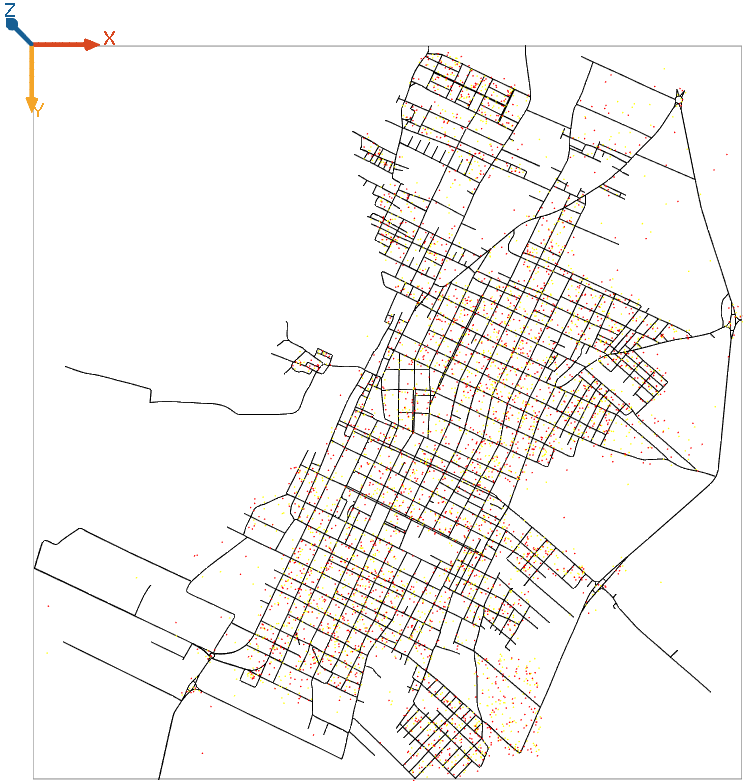
\includegraphics[width=16cm, height=10cm]{images/gama-example.png}
    \caption{Geographic view in GAMA platform.}
    \label{fig:example-gama}
\end{figure}

\section{Computational Experiments} \label{sec:computational-experiments}

The experiments were carried out on an Intel(R) Xeon(R)  CPU E5-2630 v4  processor with 10 cores of 2.20 GHz each and 64Gb of RAM. The implementation uses GAMA Platform version 1.9.2, the OSMnx Python Library~\citep{boeing:2017} 1.9.3 was used to extract the map from \gls{osm}, and the street blocks are computed using the procedure described in Section~\ref{sec:instance-generation}. Considering the robustness of the model, during the experiments, the GAMA managed to run simulations with around 80,000 agents and 500 independent simulations in the same batch in less than 4 hours with parallelism and without terminating the process due to lack of memory.
The code is available in this public repository on Github\footnote{\url{https://github.com/cvaraujo/dengue-cbrp-mabs}}.

This study explores different combinations of parameters from Table~\ref{tab:initial-pop-params} to identify the optimal configuration for each city based on the average number (min and max) of cases per week in multiple simulation runs. The precision and reliability of the results are assessed through the Pearson correlation coefficient ($r$), \gls{mae}, and the analysis of the simulated endemic channel.

\begin{table}[ht!]
\centering
\caption{Parameters for the initial state of the simulation.}
\label{tab:initial-pop-params}
\resizebox{\textwidth}{!}{%
\begin{tabular}{c|l|c}
\toprule
\textbf{Parameter} & \textbf{Description} & \textbf{Value} \\ 
\midrule
$p$ & Number of people per $m^2$ & 0.004 - 0.01 \\
$H_b$ & Number of people in block b & $p \times A_b$ \\
$H_0$ & Starting size of human population & $\sum_{b = 1}^{B} H_b$ \\
$M_h$ & Number of mosquitoes per human & 0.50 - 3.00 \\
$M_b$ & Percent of infected mosquitoes in a block without notifications & 0.05 - 0.30 \\
$M_{b}^i$ & Percent of infected mosquitoes in a block with at least one notification & 0.40 - 0.90 \\
$BS$ & Number of potential Breeding Sites & 50 - 500 \\ 
\bottomrule
\end{tabular}%
}
\end{table}

\subsection{Data Processing}\label{subsec:data-processing}

First, the objective is to establish the initial population size by computing the $p$ values.
This work calculates the area of each block of streets as a polygon using the Shapely\footnote{\url{https://shapely.readthedocs.io/en/stable/}} and Geopandas\footnote{\url{https://geopandas.org/en/stable/}} Python libraries with data imported from \gls{osm}. Since the investigation in this work focuses mainly on urban areas, and both cities have vast territorial extensions that are predominantly composed of rural areas, their overall population densities reported in \gls{ibge} are low. 
Because this study focuses on urban areas, while both municipalities have large territories predominantly composed of rural zones, their overall population densities reported by the \gls{ibge} are too low. To address this, we restrict the calculation of population density to the city center and its immediately adjacent areas. However, no population data are available at the level of blocks or neighborhoods. Therefore, we approximate the number of residents in the city centers using the number of registered electors\footnote{\url{https://international.tse.jus.br/en}} and combine this with \gls{osm}-based measurements of the urban footprint to estimate people per square meter. These estimates are used both to refine the resident population size and to define the initial population parameters for the simulation.

The choice of using a parameter ($p$) defined as persons per square meter (m\textsuperscript{2}) ensures a good level of generalization for the simulation, as the presence of this value allows the population to remain proportionally adjusted for different experiments changing the size of the city map. This can be particularly useful, for example, if we wish to simulate the evolution of dengue cases in a single neighborhood.

Based on data provided by \gls{osm}, the urban area considered in Alto Santo covers approximately 0.9~km\textsuperscript{2}, with an estimated population of 9,000 people living in the city centers. This yields a population density of $p = 0.01$ people per m\textsuperscript{2}. For Limoeiro, the approximate urban area has 8~km\textsuperscript{2} and a population of 32000, which corresponds to a value of \( p = 0.004 \) people per m\textsuperscript{2}. Since this \gls{mabs} positions the individuals within blocks, the starting human population consists of the sum of $p$ multiplied by the area of the corresponding block. For Alto Santo, using a radius of 700~m inside OSMnx, 73 street blocks are generated and the starting human population is $H_0 = 5688$. In Limoeiro, with a large urban area, the radius of 2000~m provides 563 blocks and an initial population $H_0 = 29914$. 

The starting size of the mosquito population is determined by $m = H_b \times M_h$, where the number of infected mosquitoes in the block is $M_b \times m$ for blocks without cases and $M_b^{i} \times m$ otherwise. The starting number of potential breeding sites is related to the parameter $BS$ and the blocks. For each block, if there is at least one positive case, then there is at least one breeding site. At the end of the initial scenario creation, if the breeding sites located are fewer than $BS$, then the remaining were placed in random blocks. 

The \gls{mabs} initialize using epidemiological data from a specified start date, incorporating historical notifications from the preceding week as confirmed cases within the simulation blocks.
This methodology is in line with standard public health surveillance practices. 
To validate accuracy and quality, the simulated case projections are systematically compared with actual weekly reported cases over a 90-day evaluation period (equivalent to 180 simulation cycles after initialization). The selected starting dates are selected based on epidemiological periods within a reasonable number of notifications, as explored in Section~\ref{sec:real-notifications}.

The parameters tested were $M_h = [0.5, 1, 2, 3]$, $M_b = [0.05, 0.1, 0.15, 0.2, 0.3]$, $M_b^{i} = [0.4, 0.5, 0.6, 0.7, 0.8]$, and $BS = [50, 100, 200, 300, 500]$. The analysis aggregates the results of 100 independent simulation trials for each parameter configuration and start date, ensuring statistical robustness in assessing model performance. The default maps of Alto Santo and Limoeiro consider OSMnx radius of 700~m and 2000~m, respectively. 

An independent set of initial dates was defined for each city. 
The objective of the parameter exploration is to determine the best configuration based on similarity with historical real-world data, which were mapped to the same map segment used in the simulation. 
One set of parameters is considered better than another using the number of ``wins'' for the dates on which these three criteria, in the following order of precedence, were better: (1) higher correlation between the simulated mean and the real data; (2) lower \gls{mae} between the simulated mean and the historical data; (3) number of weeks in which the real case notifications fall within the Simulation Endemic Channel, that is, the range between the highest and lowest number of simulated cases in a given week. The concept of endemic channel is used by the public health departments to assess how the number of cases in the current \gls{ew} compares with the historical in previous years. 

\subsection{Results for Alto Santo}\label{subsec:results-alto-santo}

To determine the start dates for the experiments, we selected the two years with the highest number of positive or pending notifications (2017 and 2021). The cases were then grouped by epidemiological week, as shown in Figure~\ref{fig:cases-per-week-as}. The objective is to focus on periods with the highest number of cases and consistency between adjacent weeks, while avoiding intervals with few or no cases. The experiments explore different starting dates within these periods to analyze the simulation's behavior when initiated at distinct moments along the endemic curve. Only historical notifications that can be assigned to a block in the simulation are considered, ensuring a fair comparison.

For better visualization of the results achieved by the simulator, Figure~\ref{fig:avg-result-2017-01-as} presents the results for the best configuration considering the following starting dates: \textit{(1)}~2017-01-08, \textit{(2)}~2017-01-15, \textit{(3)}~2017-01-22, \textit{(4)}~2017-01-29, \textit{(5)}~2021-05-30, and \textit{(6)}~2021-06-06. The X-axis represents the week number, the Y-axis represents the number of cases, the solid black line represents the total real notifications in the week, the dashed line represents the average number of cases across simulations with the same starting scenario, and the light gray ``$\times$'' markers represent the number of cases for a given simulation run.

\begin{figure}[!ht]
    \begin{minipage}[c]{.45\textwidth}
      \centering
      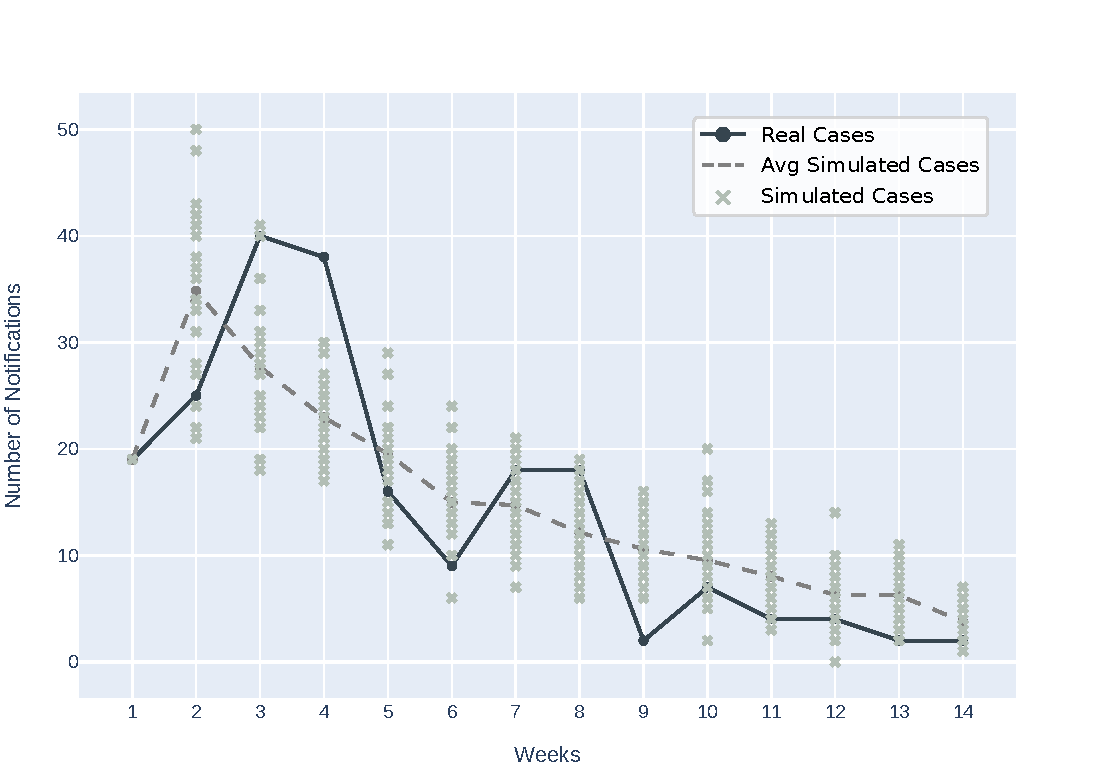
\includegraphics[scale=0.4]{images/experiments-as/AS-2017-01-08.pdf}
      \subcaption{\label{subfig:as-a} 2017-01-08}
    \end{minipage}
    \hspace{0.5cm}
    \begin{minipage}[c]{.45\textwidth}
        \centering
        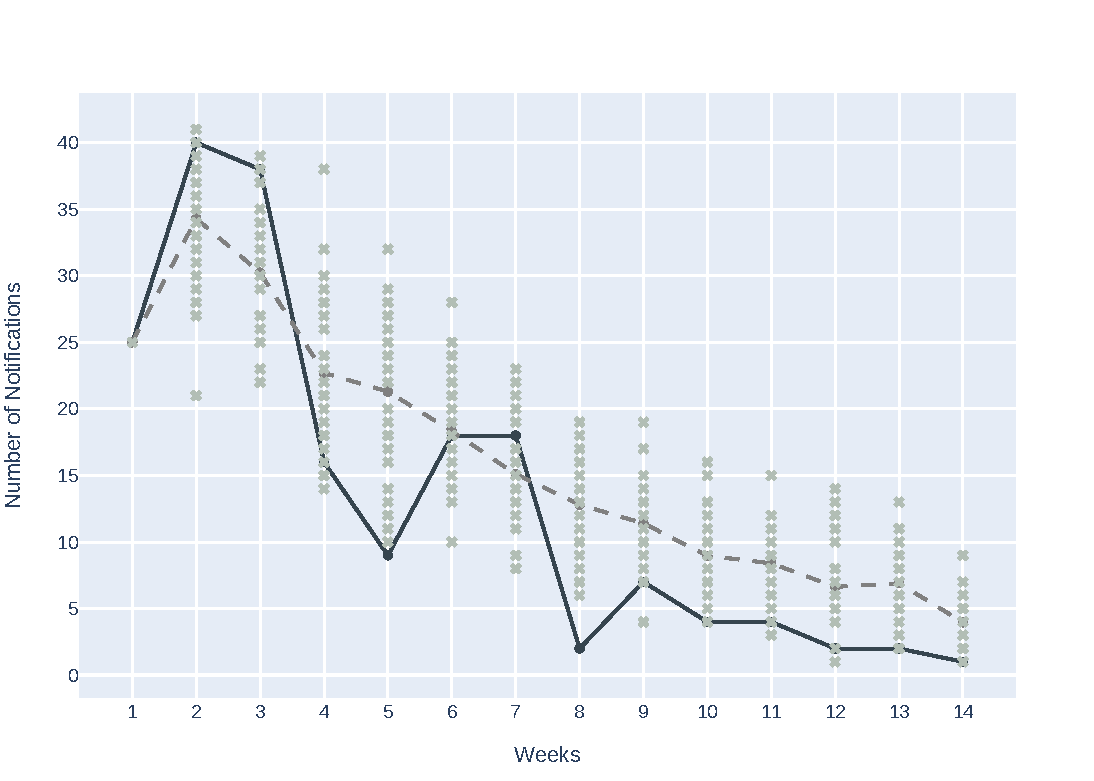
\includegraphics[scale=0.4]{images/experiments-as/AS-2017-01-15.pdf}
        \subcaption{\label{subfig:as-b} 2017-01-15}
    \end{minipage}
    \\
    \begin{minipage}[c]{.45\textwidth}
        \centering
        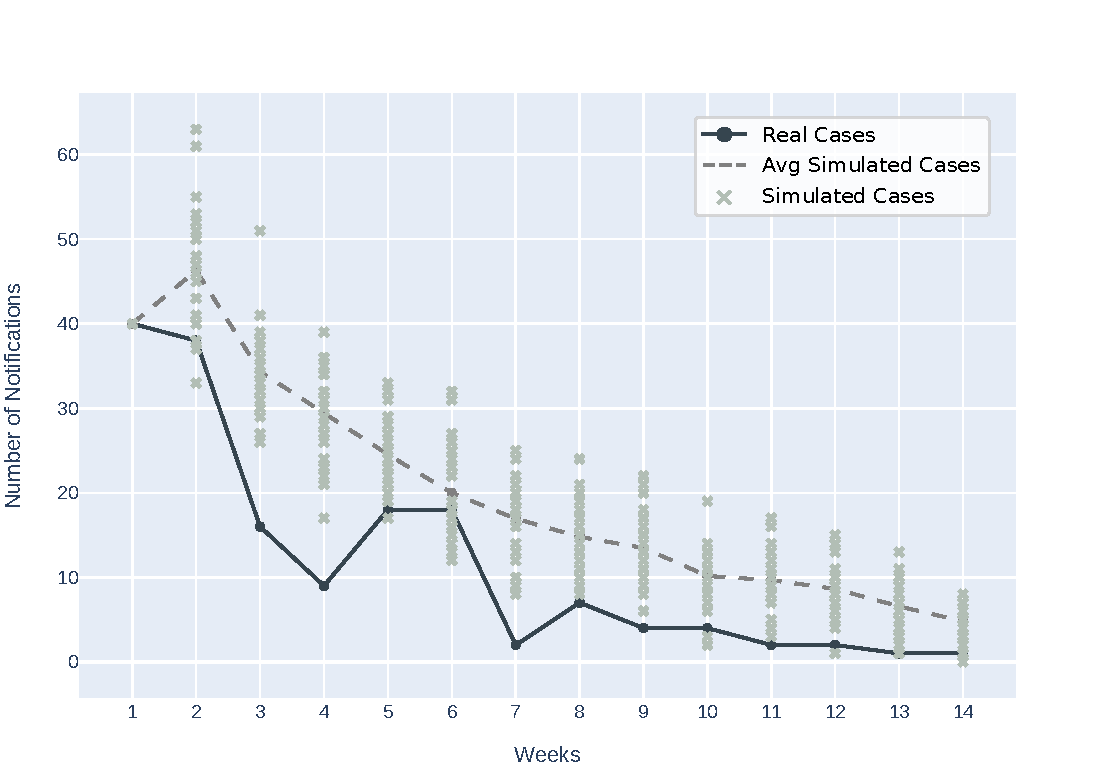
\includegraphics[scale=0.4]{images/experiments-as/AS-2017-01-22.pdf}
        \subcaption{\label{subfig:as-c} 2017-01-22}
      \end{minipage}
      \hspace{0.5cm}
      \begin{minipage}[c]{.45\textwidth}
          \centering
          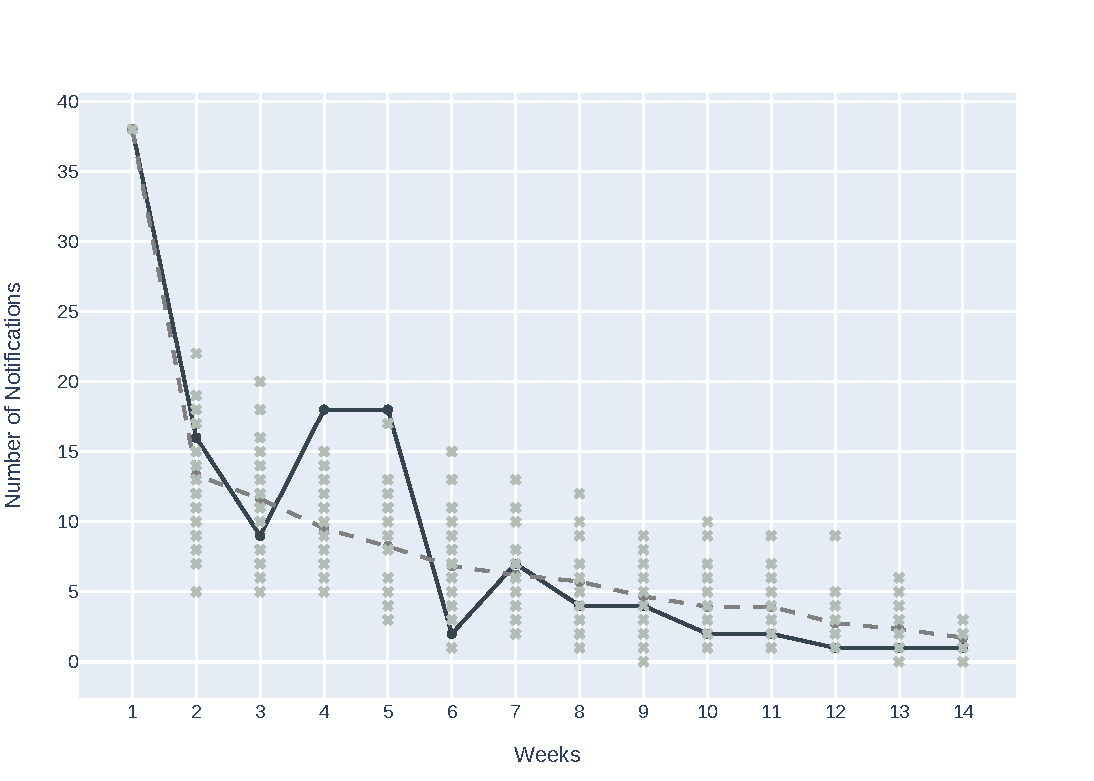
\includegraphics[scale=0.4]{images/experiments-as/AS-2017-01-29.pdf}
          \subcaption{\label{subfig:as-d} 2017-01-29}
    \end{minipage}
    \\
    \begin{minipage}[c]{.45\textwidth}
        \centering
        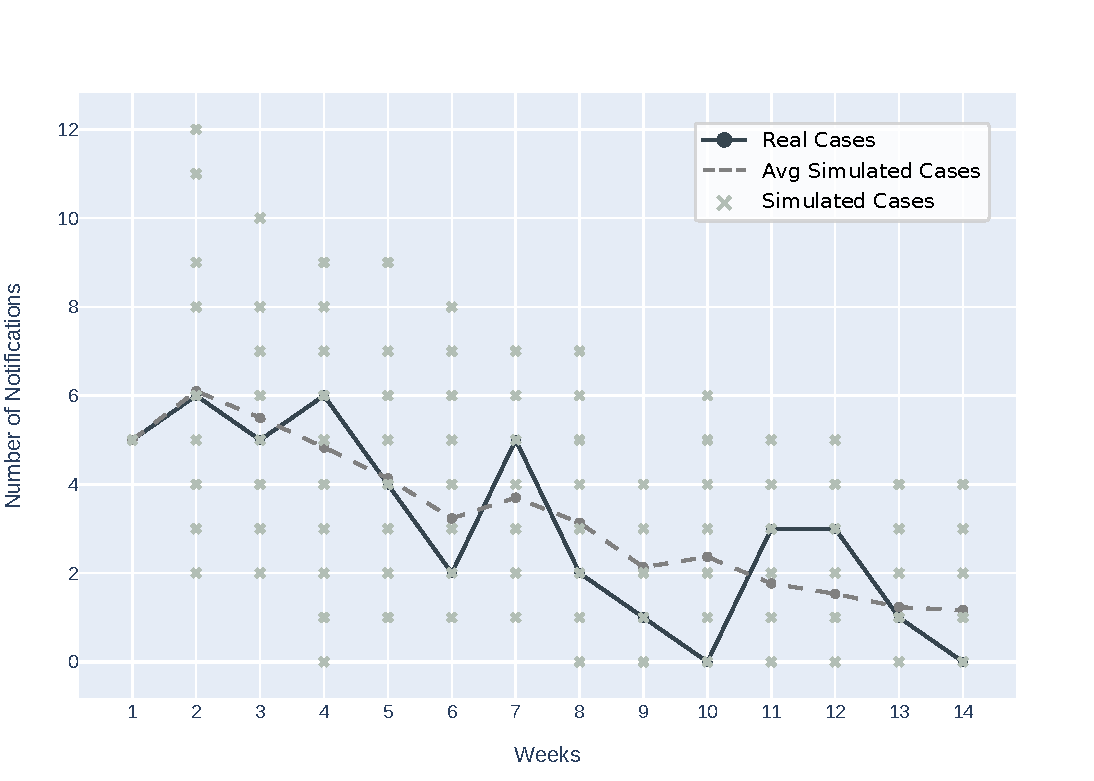
\includegraphics[scale=0.4]{images/experiments-as/AS-2021-05-30.pdf}
        \subcaption{\label{subfig:as-e} 2021-05-30}
      \end{minipage}
      \hspace{0.5cm}
      \begin{minipage}[c]{.45\textwidth}
        \centering
        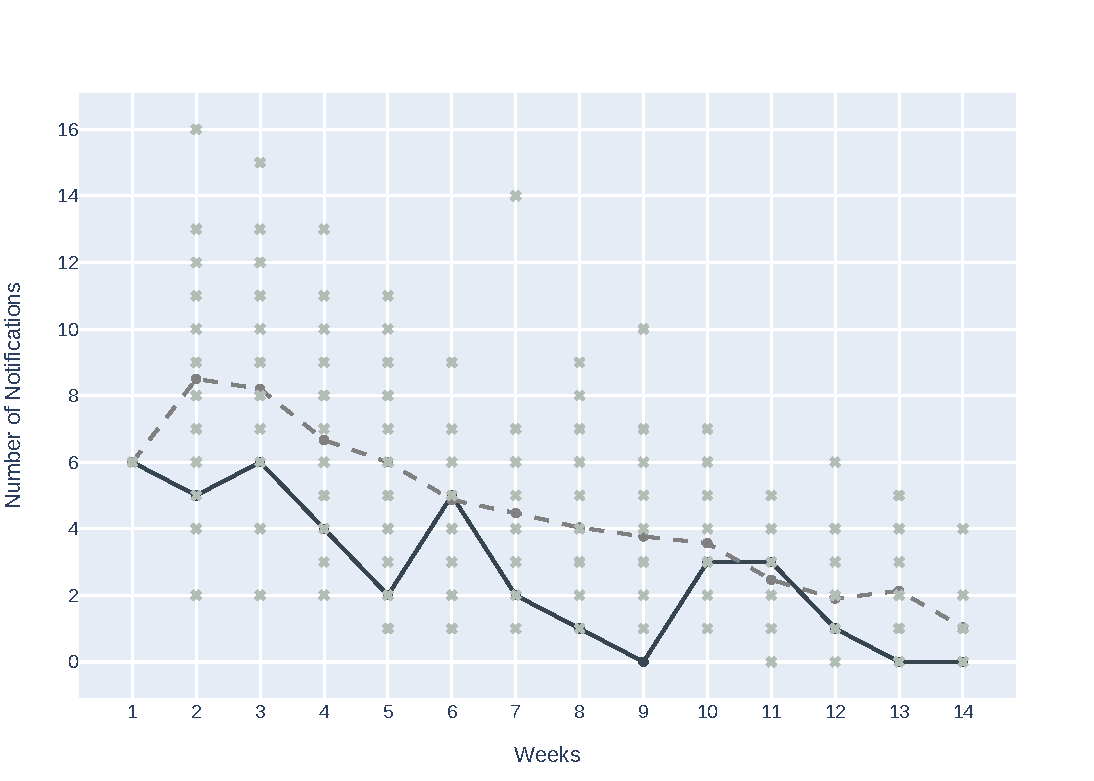
\includegraphics[scale=0.4]{images/experiments-as/AS-2021-06-06.pdf}
        \subcaption{\label{subfig:as-f} 2021-06-06}
      \end{minipage}
    \caption{\label{fig:avg-result-2017-01-as} Comparison of simulation and real cases from \textit{Alto Santo} for different starting dates.}
\end{figure}

The results represented in Figure~\ref{fig:avg-result-2017-01-as} correspond to the variable parameters $M_h = 1$, $BS = 50$, $M_b = 0.05$ and $M_b^{i} = 0.4$, which is the combination that achieved the best results considering the highest correlation values ($r$) among all configurations for \textit{Alto Santo}. More detailed information on these results is discussed later in this section.
%
Table~\ref{tab:statistical-data-as} shows the values of \gls{mae}, the correlation of the average simulated cases with the real notification ($r$) and the confidence interval (CI), in addition to the graphical results presented in Figure~\ref{fig:avg-result-2017-01-as}.

\begin{table}[!ht]
\centering
\caption{Statistical values from the best configuration - \textit{Alto Santo} city.}
\label{tab:statistical-data-as}
\small{%
\begin{tabular}{lrrrr}
\toprule
  \multicolumn{1}{c}{\textbf{Date}} &
  \multicolumn{1}{c}{\textbf{MAE}} &
  \multicolumn{1}{c}{\textbf{$r$}} &
  \multicolumn{1}{c}{\textbf{$CI_{min}$}} &
  \multicolumn{1}{c}{\textbf{$CI_{max}$}} \\ \midrule
2017-01-08 & 5.67  & \textbf{0.83} & 0.61  & 0.94 \\
2017-01-15 & 5.20  & \textbf{0.93} & 0.82  & 0.97 \\
2017-01-22 & 8.40  & \textbf{0.90}  & 0.75  & 0.96 \\
2017-01-29 & 2.80  & \textbf{0.92} & 0.80  & 0.97 \\
2021-05-30 & 0.94  & \textbf{0.84} & 0.62  & 0.94 \\
2021-06-06 & 1.92  & \textbf{0.77} & 0.49  & 0.91 \\ \bottomrule
\end{tabular}%
}
\end{table}

All experiments strongly correlate with real cases, achieving correlation coefficients of at least $0.77$ with positive confidence intervals. This strong correlation indicates that the average number of simulated cases per week closely matches the real number of cases. The endemic channel generated in each image of Figure~\ref{fig:avg-result-2017-01-as} has a difference of at most 10 cases from the real notifications when they are outside the endemic channel for a given \gls{ew}, which represents a small deviation from reality.

\subsection{Results for Limoeiro}\label{subsec:results-limoeiro}

The years 2019 and 2020 are selected for \textit{Limoeiro} city, and the number of cases per week is shown in Figure~\ref{fig:cases-per-week-limoeiro}. 
Figure~\ref{fig:avg-result-lim} presents the results for the following starting dates: \textit{(1)}~2019-04-14, \textit{(2)}~2019-05-05, \textit{(3)}~2020-06-21, \textit{(4)}~2020-07-05, \textit{(5)}~2020-07-19, and \textit{(6)}~2020-07-26. 
Due to the extreme difference in the number of cases between the two years for \textit{Limoeiro}, where 2020 has more than 1000 notifications than 2019, it was not possible to define a set of parameters that fit well for both years with such different samples and behavior.
Figures~\ref{subfig:lim-a} and~\ref{subfig:lim-b} show the best results obtained with the parameters $M_h = 0.5$, $BS = 100$, $M_b = 0.05$ and $M_b^{i} = 0.4$. Figures~\ref{subfig:lim-c} to~\ref{subfig:lim-f} present the results with the following parameters set $M_h = 1$, $BS = 500$, $M_b = 0.20$ and $M_b^{i} = 0.9$.

\begin{figure}[!ht]
    \begin{minipage}[c]{.45\textwidth}
      \centering
      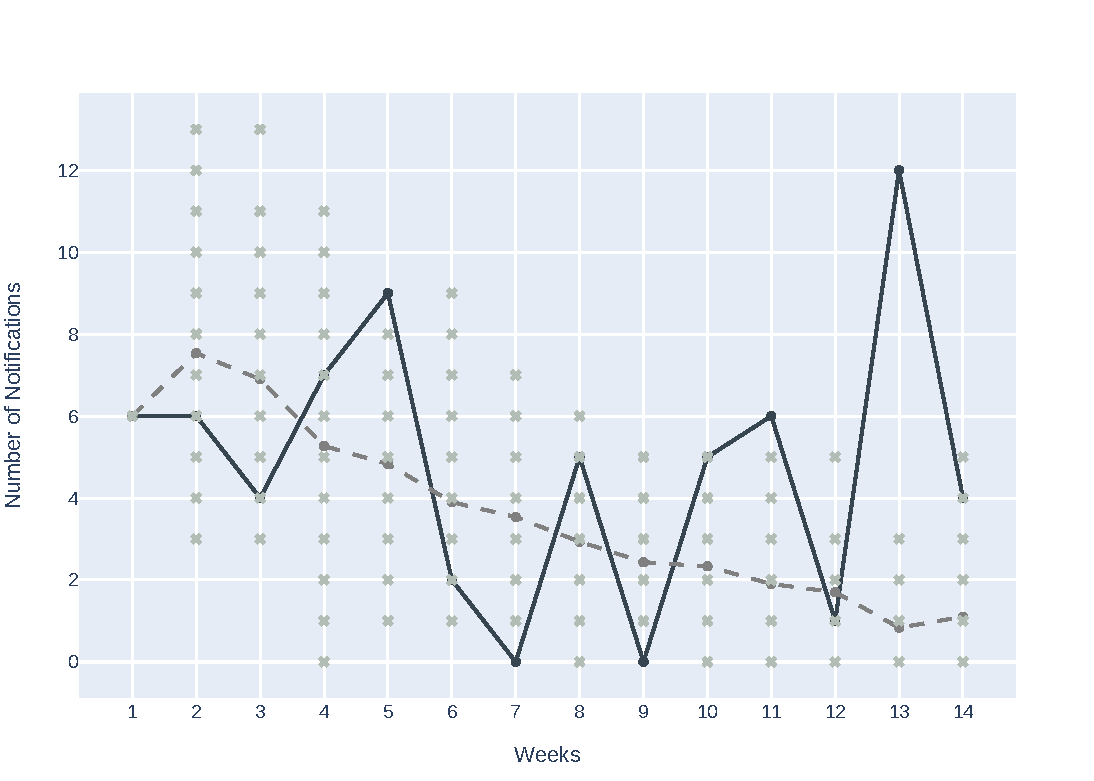
\includegraphics[scale=0.4]{images/experiments-lim/LIM-2019-04-14.pdf} \\
      \subcaption{\label{subfig:lim-a} 2019-04-14}
    \end{minipage}
    \hspace{0.5cm}
    \begin{minipage}[c]{.45\textwidth}
        \centering
        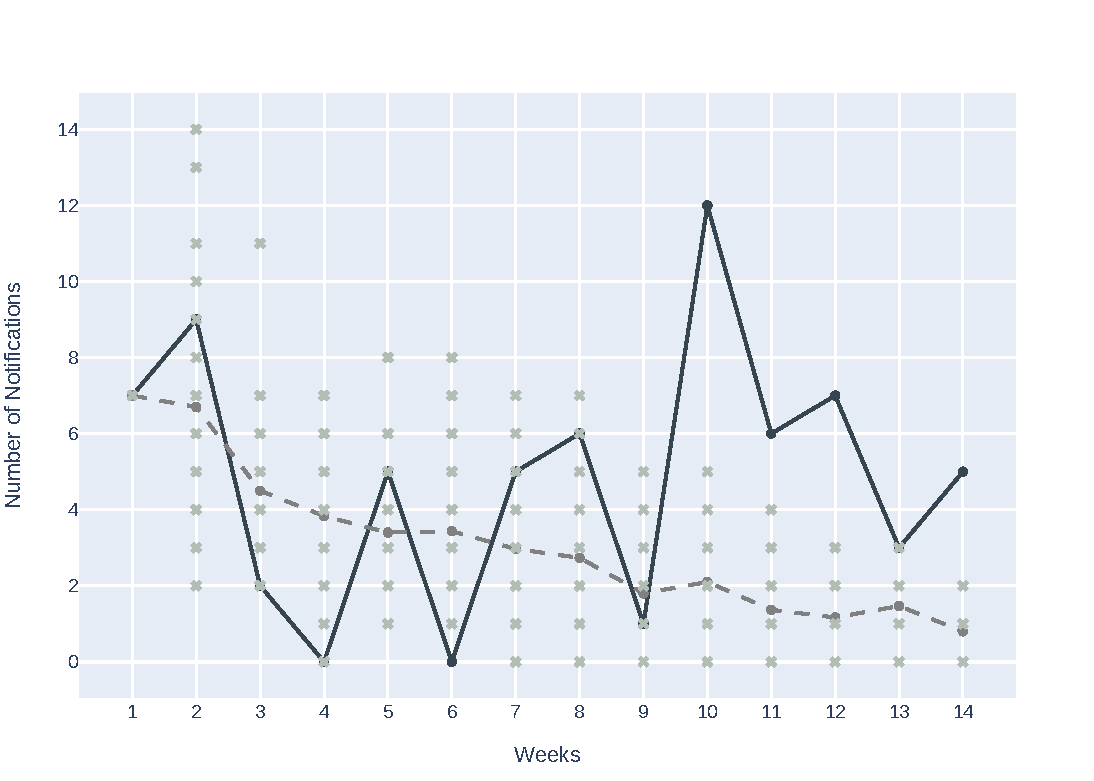
\includegraphics[scale=0.4]{images/experiments-lim/LIM-2019-05-05.pdf} \\
        \subcaption{\label{subfig:lim-b} 2019-05-05}
    \end{minipage}
    \\
    \begin{minipage}[c]{.45\textwidth}
        \centering
        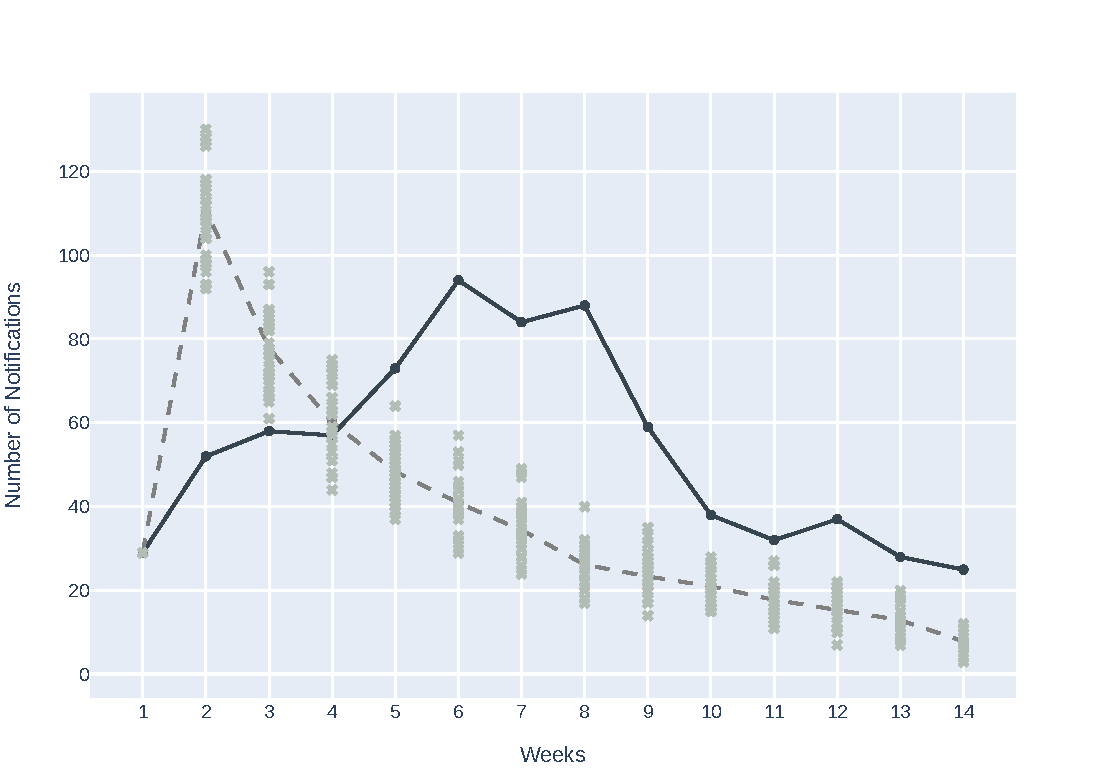
\includegraphics[scale=0.4]{images/experiments-lim/LIM-2020-06-21.pdf} \\
        \subcaption{\label{subfig:lim-c} 2020-06-21}
      \end{minipage}
    \hspace{0.5cm}
    \begin{minipage}[c]{.45\textwidth}
          \centering
          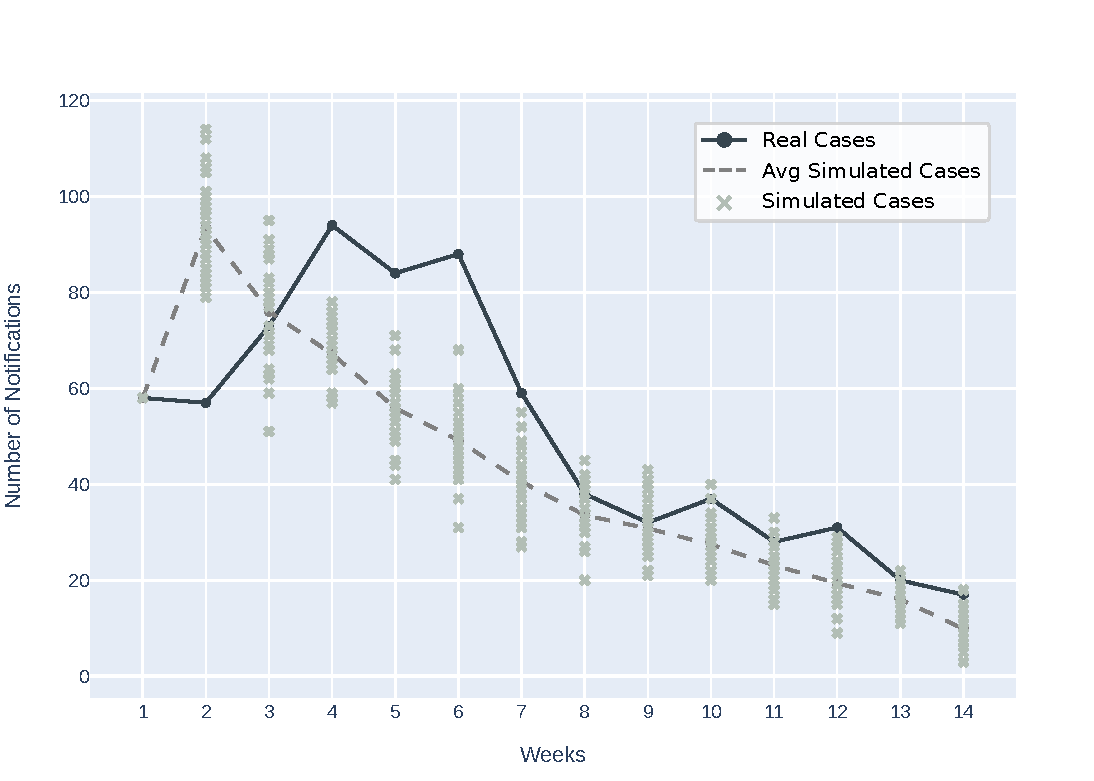
\includegraphics[scale=0.4]{images/experiments-lim/LIM-2020-07-05.pdf} \\
          \subcaption{\label{subfig:lim-d} 2020-07-05}
    \end{minipage}
    \\
    \begin{minipage}[c]{.45\textwidth}
        \centering
        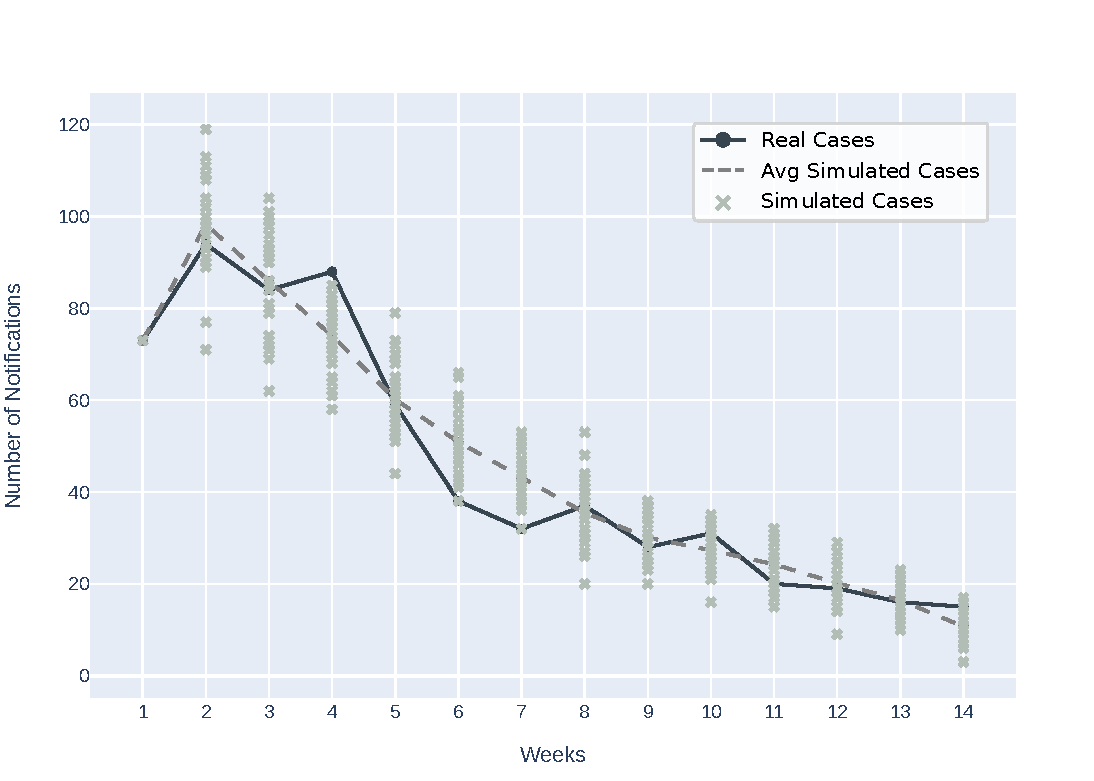
\includegraphics[scale=0.4]{images/experiments-lim/LIM-2020-07-19.pdf} \\
        \subcaption{\label{subfig:lim-e} 2020-07-19}
      \end{minipage}
    \hspace{0.5cm}
    \begin{minipage}[c]{.45\textwidth}
        \centering
        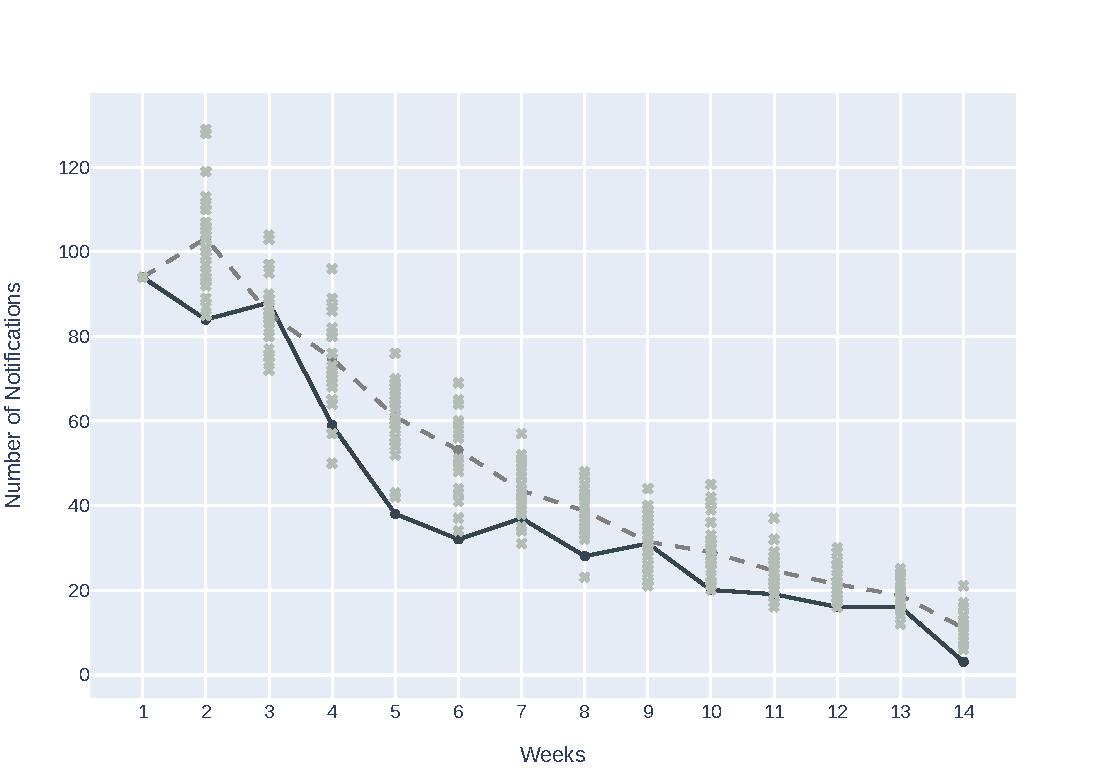
\includegraphics[scale=0.4]{images/experiments-lim/LIM-2020-07-26.pdf} \\
        \subcaption{\label{subfig:lim-f} 2020-07-26}
      \end{minipage}
    \caption{\label{fig:avg-result-lim} Comparison of simulation and real cases from \textit{Limoeiro} for different starting dates.}
\end{figure}

Table~\ref{tab:statistical-data-lim} shows the values of \gls{mae}, the correlation of the average simulated cases with the real notification ($r$), and the confidence interval of the results presented in Figures~\ref{fig:avg-result-lim}.

\begin{table}[!ht]
\centering
\caption{Statistical values from the best configuration - \textit{Limoeiro} city.}
\label{tab:statistical-data-lim}
\small{%
\begin{tabular}{lrrrr}
\toprule
  \multicolumn{1}{c}{\textbf{Date}} &
  \multicolumn{1}{c}{\textbf{MAE}} &
  \multicolumn{1}{c}{\textbf{$r$}} &
  \multicolumn{1}{c}{\textbf{$CI_{min}$}} &
  \multicolumn{1}{c}{\textbf{$CI_{max}$}} \\ \midrule
2019-04-14 & 2.99  & 0.06          & -0.41 & 0.51 \\
2019-05-05 & 3.28  & 0.09          & -0.38 & 0.53 \\
2020-06-21 & 27.97 & 0.30          & -0.18 & 0.67 \\
2020-07-05 & 13.90 & \textbf{0.76} & 0.45  & 0.90 \\
2020-07-19 & 4.49  & \textbf{0.97} & 0.93  & 0.99 \\
2020-07-26 & 9.27  & \textbf{0.96} & 0.90  & 0.99 \\ \bottomrule
\end{tabular}%
}
\end{table}

In 2019, the analysis of \textit{Limoeiro} City’s epidemiological data revealed a weak correlation (values approaching zero), as indicated by the experimental results. However, the associated \gls{mae} metrics were modest, ranging from $2.99$ to $3.28$. Figures~\ref{subfig:lim-a} and~\ref{subfig:lim-b} illustrate the weekly case distribution, highlighting irregular temporal patterns despite the low overall incidence (with a peak of 12 notifications in the highest week). In particular, only 4 of the 14 analyzed \gls{ew} exceeded the boundaries of the simulated endemic channel.

Discrepancies between observed and expected case counts were predominantly minor (1-2 cases), except for the $10^{th}$ and $13^{th}$ weeks, which each recorded 12 notifications and deviated by 9 cases from the channel’s upper limit. This suggests that while the statistical correlation was weak, most of the weekly case counts aligned with or remained close to the endemic channel. The results show that even in low-incidence settings, localized fluctuations can occur without systematically breaching expected epidemiological thresholds.

Figures~\ref{subfig:lim-c} and~\ref{subfig:lim-d} represent two simulations started two weeks apart. In the first scenario, starting in 2020-06-21, the model yields a weak correlation $(r = 0.3)$, as it anticipates a case peak in the initial weeks, while the observed data show a delayed surge in the sixth week. This temporal misalignment probably reflects limitations in model calibration, including insufficient historical data and an inability to integrate time-dependent variables that influence case trajectories.

In contrast, the second simulation, initialized on 2020-07-19, two weeks after the outbreak start date of 2020-07-05, achieved a much stronger correlation with observed data ($r = 0.76$) and a positive confidence interval (CI), indicating substantially improved alignment with real trends. The later start likely allowed the model to capture critical early-phase information, enhancing predictive accuracy. This outcome illustrates the sensitivity of our dengue spread model to the choice of initial conditions: applying the same parameter set with starting dates only 15 days apart shifted the correlation from $0.30$ to $0.76$ during a continuous outbreak season. It also suggests the value of extending the framework to incorporate dynamic seasonal behaviors.


Figures~\ref{subfig:lim-e}--\ref{subfig:lim-f}  demonstrate near-perfect correlation coefficients ($r = 0.97$ and $r = 0.96$, respectively), reflecting an exceptional alignment between simulated and observed case trends. These simulations were initialized during peak cases in incidence periods for both cities, the highest recorded in the notification dataset. The proximity of these starting dates to the epidemiological peak likely allowed the model to capture critical transmission dynamics, resulting in highly accurate projections. This outcome confirms robustness when calibrated during periods of increased disease activity, where the underlying patterns may be more pronounced and predictable.

\subsection{Sensitivity Analysis}

This experiment evaluated the influence of a subset of simulation parameters, identified as fitted in Table~2, by assessing their isolated impact on disease propagation. In each test, all parameters were held at their default values except for the one under analysis, which was systematically varied. Specifically, we considered the following sets of values: $\delta = \{0.03, 0.06, 0.12, 0.24, 0.48\}$ for the mortality rate in the aquatic phase, $\phi = \{0.01, 0.02, 0.16, 0.40, 0.80\}$ for the daily oviposition rate, and $\mu = \{0.01, 0.02, 0.16, 0.40, 0.80\}$ for the mortality rate in the adult phase. For each parameter value, we performed 100 independent runs of 180 cycles (approximately 14 weeks).

The sensitivity analysis was conducted for both cities, using two distinct dates: 2017-01-15 for Alto Santo and 2020-07-19 for Limoeiro. These dates were chosen because they correspond to cases with the highest \gls{mae} in the previous experiment, thereby providing challenging conditions for model performance. The population parameters from Table~4 were set according to the configurations that had yielded the best correlation for each city and date in the earlier experiment.

Figure~\ref{fig:sensitivity-analysis-delta} shows the results for the aquatic-phase mortality rate ($\delta$). The textured curves depict the weekly average of simulated cases for each $\delta$ value, and the solid black curve with markers is the observed series. The responses differ by city: in Limoeiro, the curves nearly overlap across the horizon, suggesting limited sensitivity of transmission to $\delta$ within the 14-week window. In Alto Santo, the curves are more distinct and non-monotonic. Higher $\delta$ does not consistently reduce cases: for example, $\delta=0.48$ produces a higher mid-season peak than $\delta \in \{0.06,0.12,0.24\}$. Although $\delta=0.03$ (lowest aquatic mortality) yields the largest first-week peak, it is subsequently overtaken by $\delta=0.48$, which later converges to among the lowest case counts near the end of the simulation.

This counterintuitive pattern may suggest that containment measures related to eliminating breeding sites may not be as effective in the short-run as one might expect, as it is currently one of the most employed actions in Brazil municipalities. To rule out Monte-Carlo noise, we repeated the experiment with 500 runs instead of 100 and obtained similar averages, indicating that the effect is not due to insufficient sampling. The precise mechanism warrants further investigation, but these results caution against assuming a simple, monotonic relationship between larval-stage mortality and short-horizon case counts in this model.


\begin{figure}[h!]
    \begin{minipage}[c]{.45\textwidth}
      \centering
      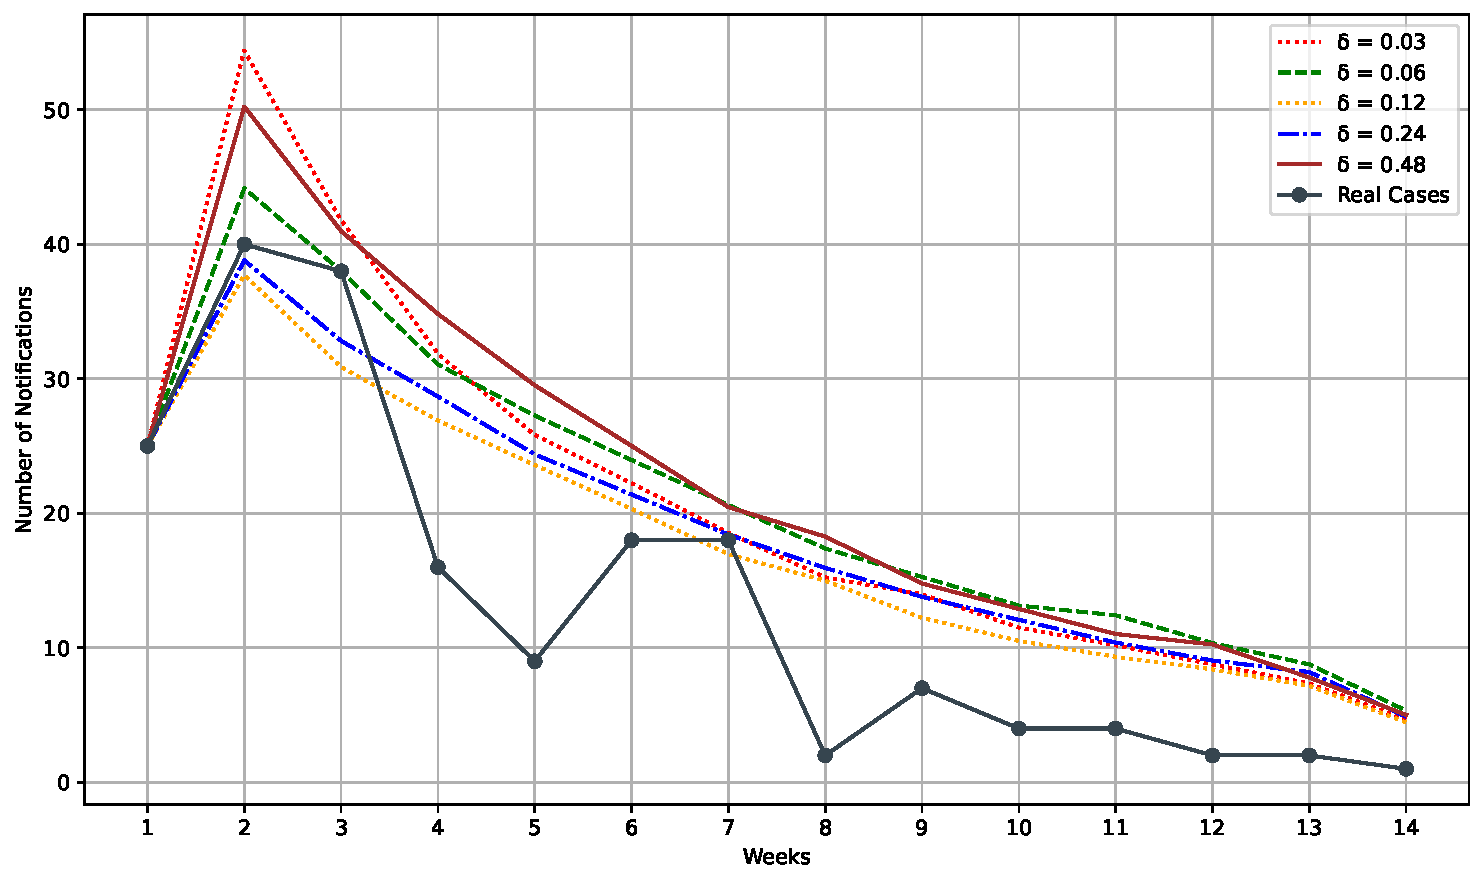
\includegraphics[scale=0.3]{images/parameters-experiments/AS_2017-01-15_bs_aquatic_phase_mortality_rate.pdf} \\
      \subcaption{\label{fig:sensitivity-analysis-delta-as}Results for Alto Santo}
    \end{minipage}
    \hspace{0.5cm}
    \begin{minipage}[c]{.45\textwidth}
        \centering
        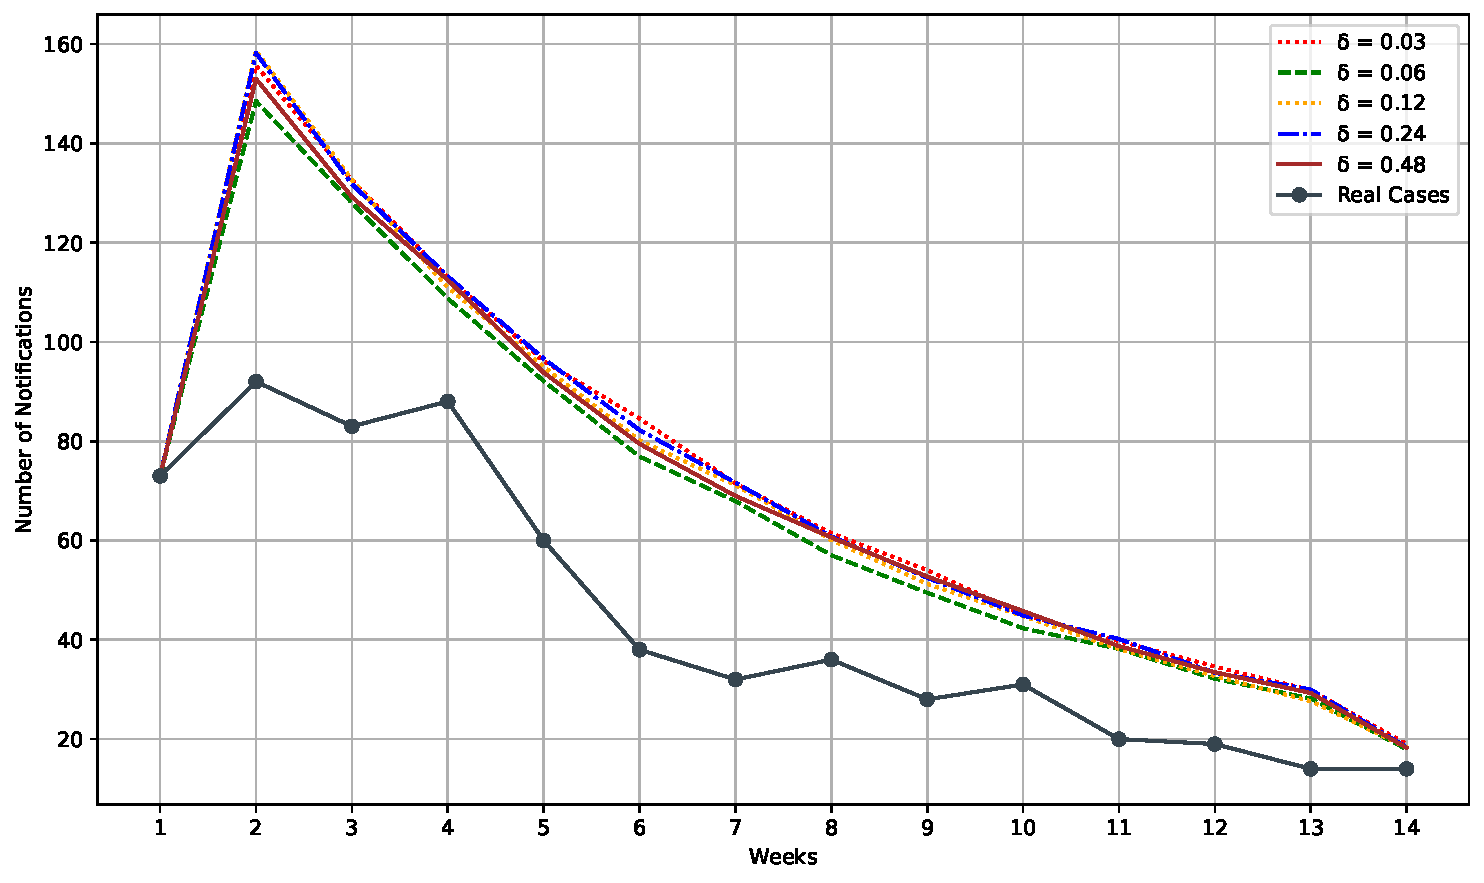
\includegraphics[scale=0.3]{images/parameters-experiments/LN_2020-07-19_bs_aquatic_phase_mortality_rate.pdf} \\
        \subcaption{\label{fig:sensitivity-analysis-delta-ln}Results for Limoeiro}
    \end{minipage}
    \caption{\label{fig:sensitivity-analysis-delta} Results for the mortality rate in aquatic phase ($\delta$) parameter.}
\end{figure}

Figure~\ref{fig:sensitivity-analysis-phi} reports the sensitivity to the daily oviposition rate ($\phi$). The patterns largely mirror those observed for $\delta$: in Limoeiro, the average trajectories for different $\phi$ values are closely aligned across the 14-week window, indicating low short-horizon sensitivity. In Alto Santo, the responses are more spreaded and again non-monotonic, with higher $\phi$ not invariably producing larger case counts. As with the previous parameter, these unexpected dynamics indicate the need for further investigation to identify the factors that may be influencing such behavior.



\begin{figure}[h!]
    \begin{minipage}[c]{.45\textwidth}
      \centering
      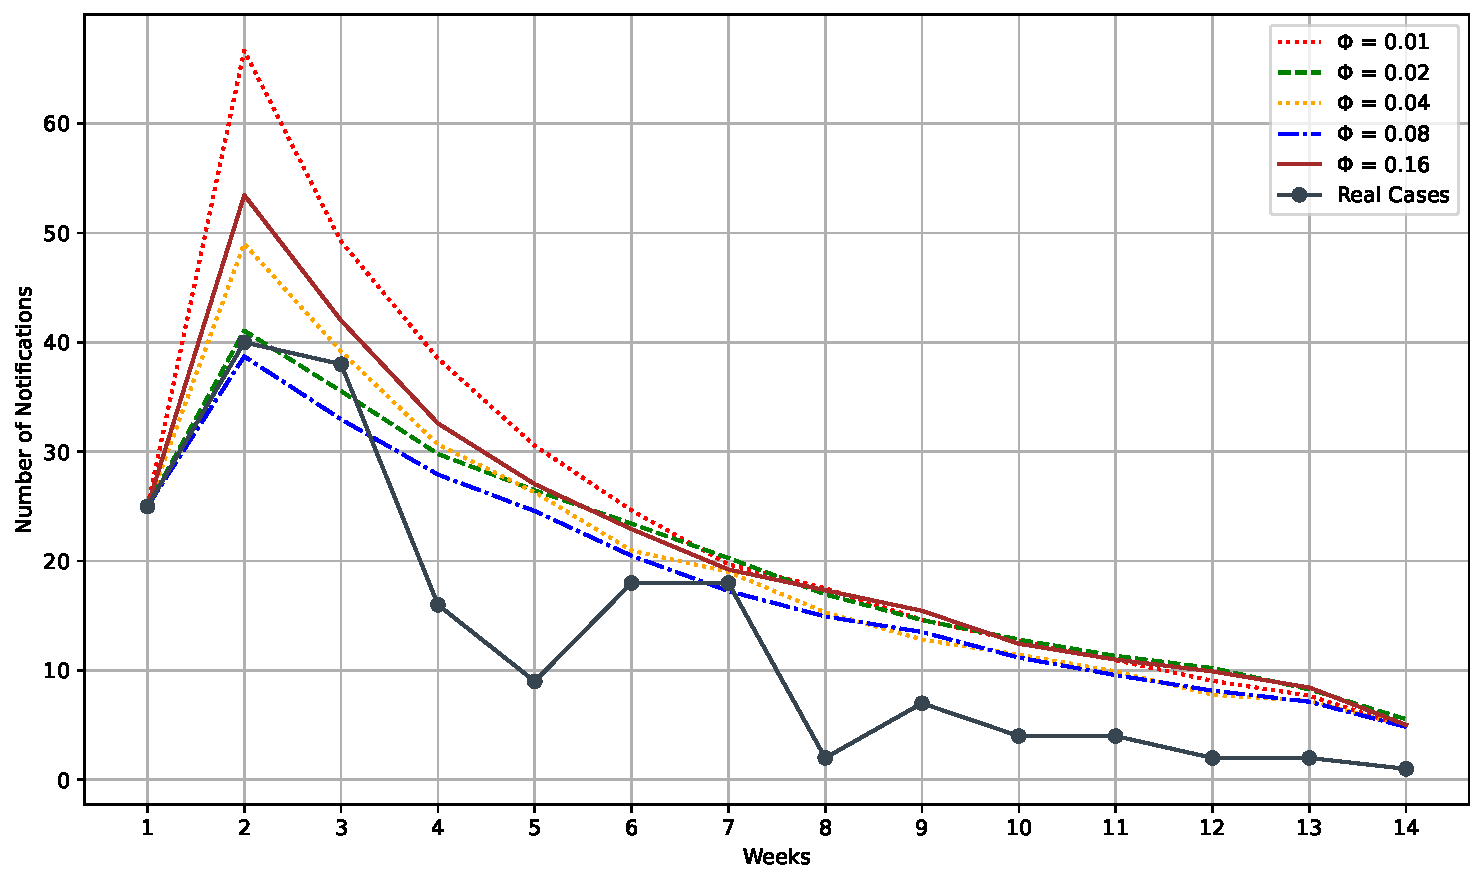
\includegraphics[scale=0.3]{images/parameters-experiments/AS_2017-01-15_mosquitoes_oviposition_rate.pdf} \\
      \subcaption{\label{fig:sensitivity-analysis-phi-as}Results for Alto Santo}
    \end{minipage}
    \hspace{0.5cm}
    \begin{minipage}[c]{.45\textwidth}
        \centering
        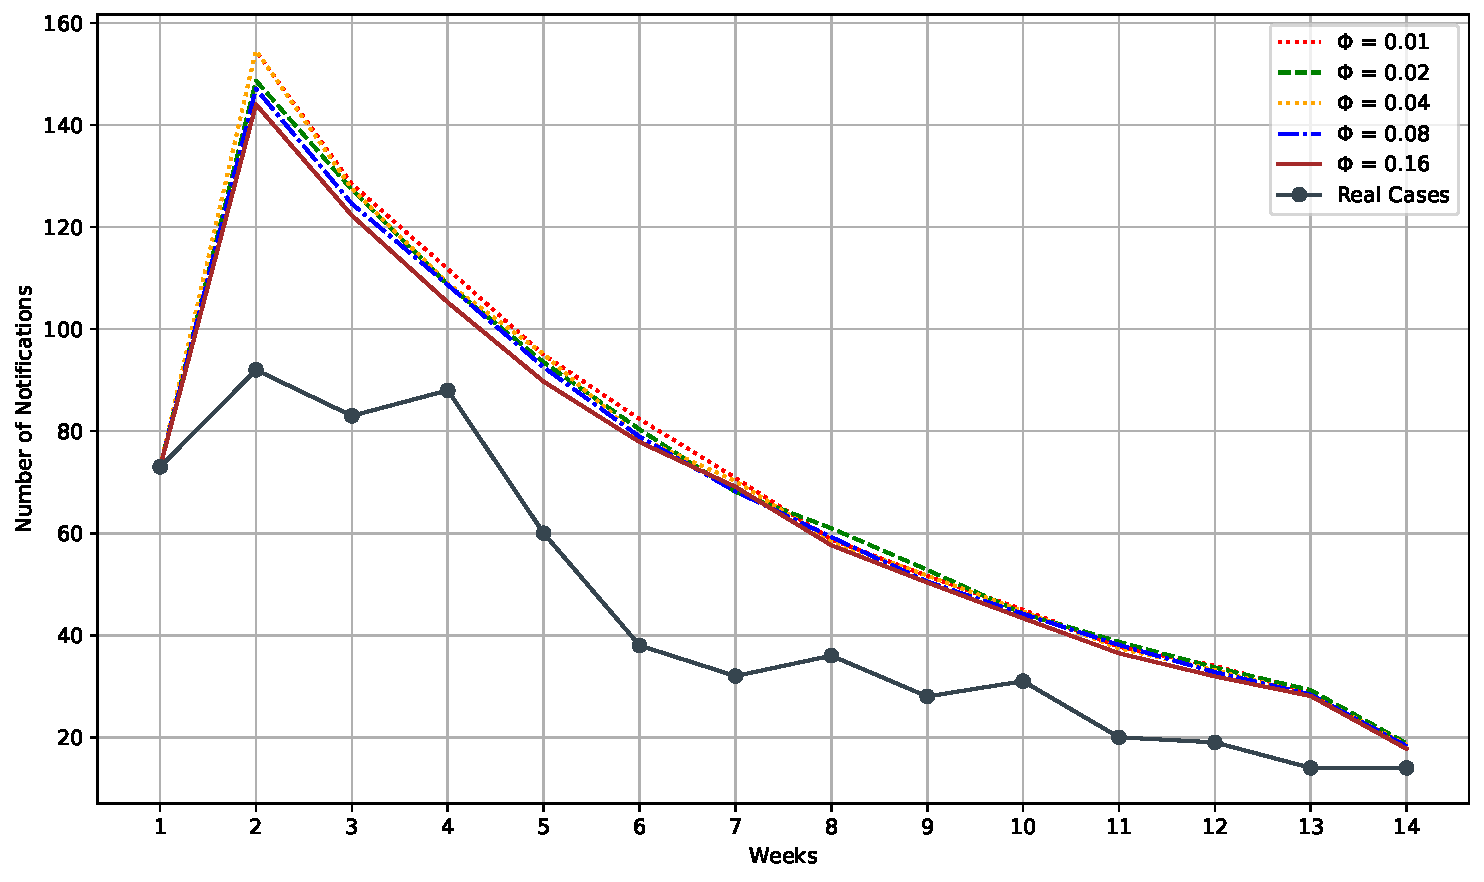
\includegraphics[scale=0.3]{images/parameters-experiments/LN_2020-07-19_mosquitoes_oviposition_rate.pdf} \\
        \subcaption{\label{fig:sensitivity-analysis-phi-ln}Results for Limoeiro}
    \end{minipage}
    \caption{\label{fig:sensitivity-analysis-phi} Results for the daily oviposition rate ($\phi$) parameter.}
\end{figure}

By contrast, the results for the adult-phase mortality rate ($\mu$), shown in Figure~\ref{fig:sensitivity-analysis-mu}, are markedly more consistent. In both Limoeiro and Alto Santo, the average trajectories decline monotonically as $\mu$ increases. Notably, for $\mu=0.16$ the simulated incidence falls to near zero by about the fourth week in both cities, highlighting that increasing adult mosquito mortality has a strong short-term suppressive effect on transmission. 


\begin{figure}[h!]
    \begin{minipage}[c]{.45\textwidth}
      \centering
      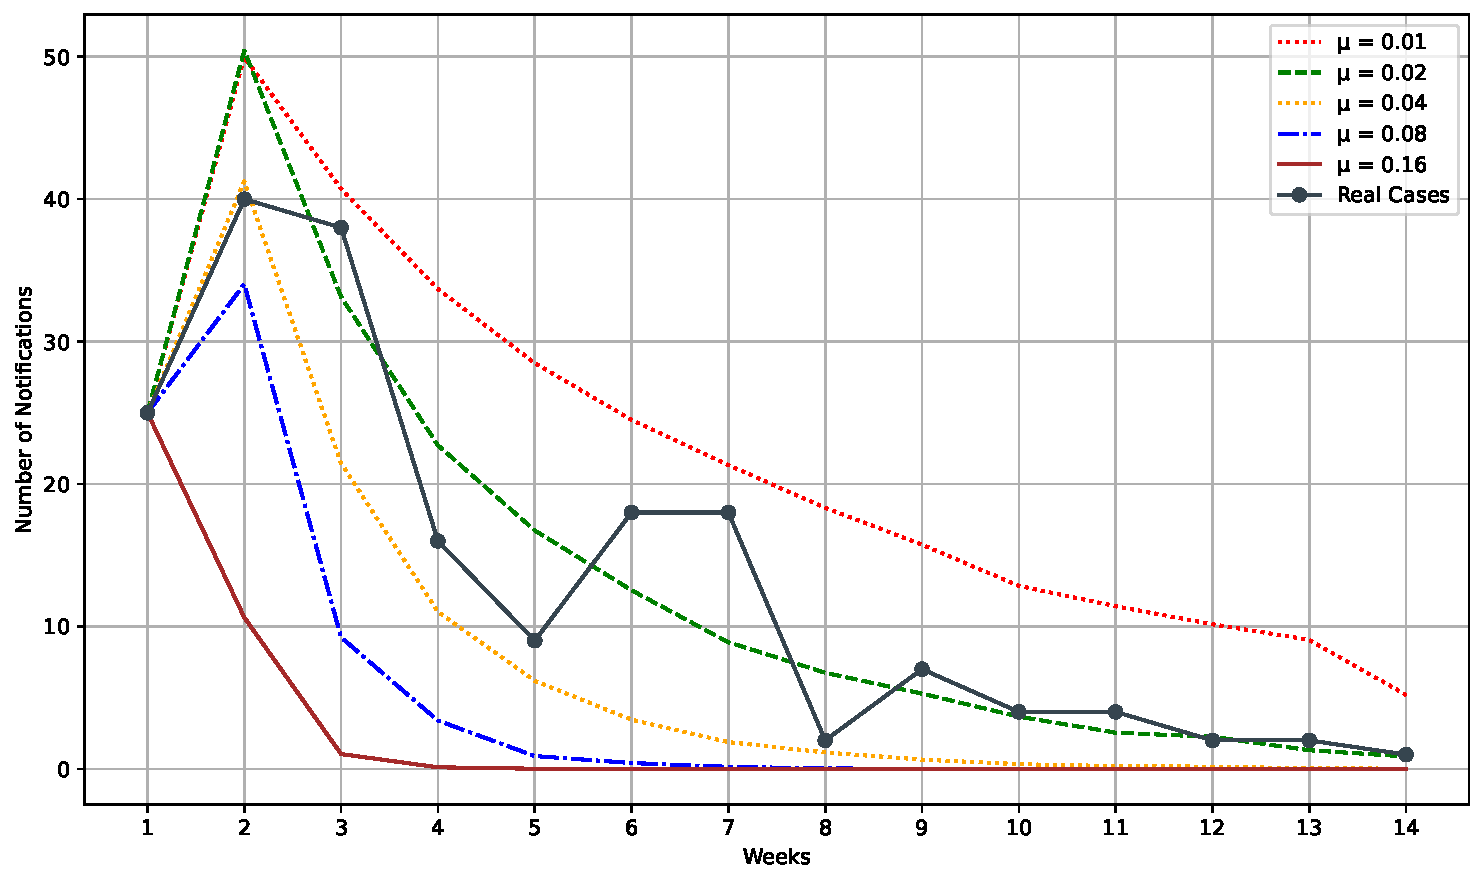
\includegraphics[scale=0.3]{images/parameters-experiments/AS_2017-01-15_mosquitoes_death_rate.pdf} \\
      \subcaption{\label{fig:sensitivity-analysis-mu-ln}Results for Alto Santo}
    \end{minipage}
    \hspace{0.5cm}
    \begin{minipage}[c]{.45\textwidth}
        \centering
        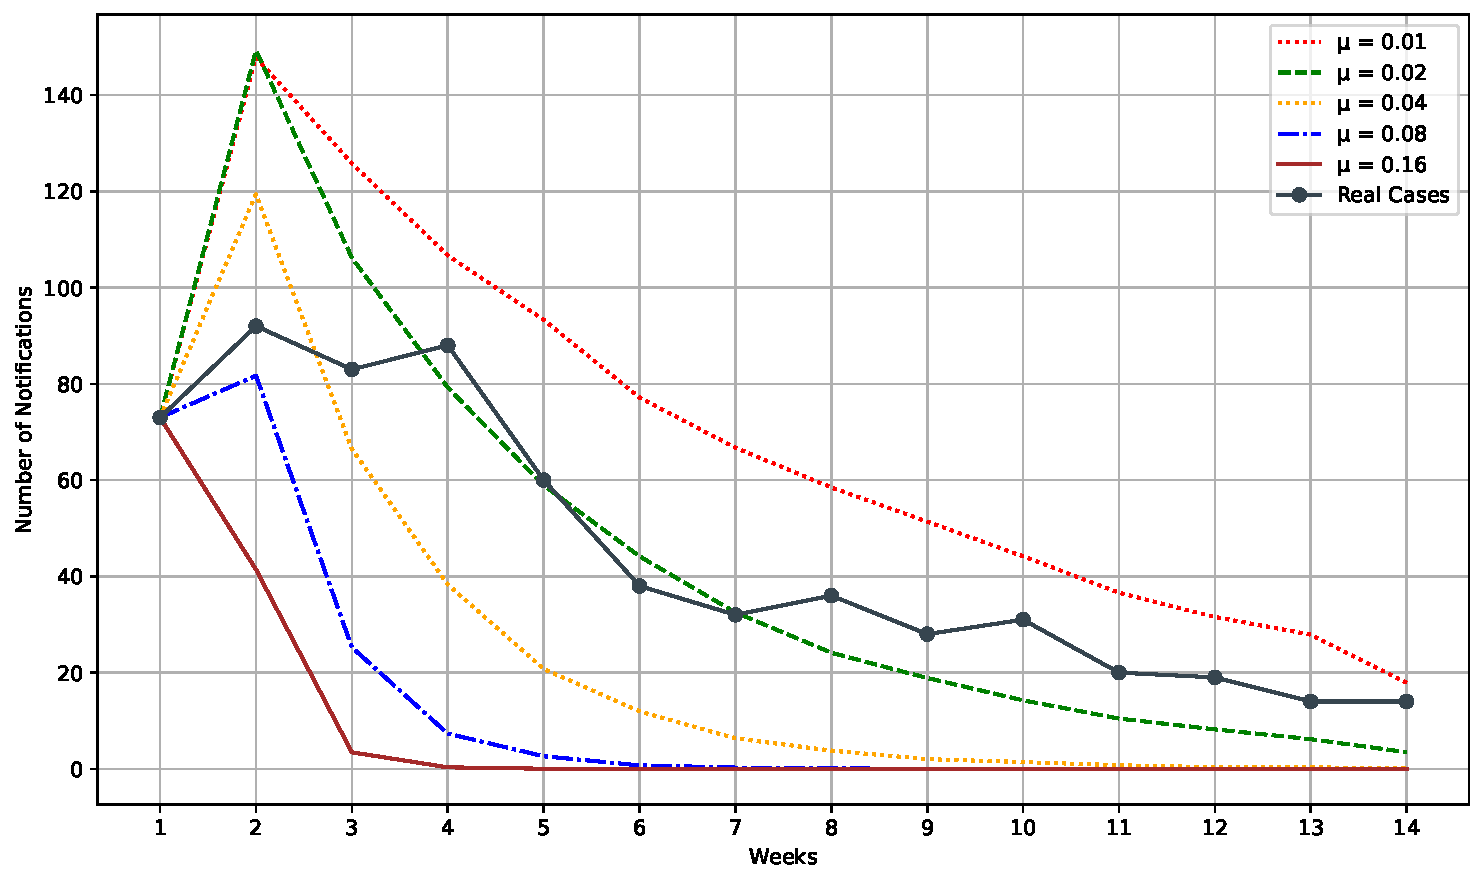
\includegraphics[scale=0.3]{images/parameters-experiments/LN_2020-07-19_mosquitoes_death_rate.pdf} \\
        \subcaption{\label{fig:sensitivity-analysis-mu-ln}Results for Limoeiro}
    \end{minipage}
    \caption{\label{fig:sensitivity-analysis-mu}Results for the mortality rate in adult phase ($\mu$) parameter}
\end{figure}


\subsection{Results Aggregated by City Block}
We evaluate block-level accuracy for Alto Santo and Limoeiro over the same 90-day horizon used in Sections~\ref{subsec:results-alto-santo}–\ref{subsec:results-limoeiro}. For each start date, Table~\ref{tab:cases-per-block} reports: (i) the city, (ii) the start date, (iii) the Mean Absolute Error (MAE) between observed cases and the average simulated cases per block at day 90, and (iv) the share of blocks whose observed cases lie within the simulated endemic channel (“Correct Blocks”). To avoid degenerate comparisons, blocks with no dengue notifications across the historical record were excluded.

In Alto Santo, MAE ranges from 1.52 to 2.75, with 86–94\% of blocks correctly captured by the endemic channel; in Limoeiro, MAE ranges from 0.80 to 2.01, with at least 85\% of blocks correctly captured. These results indicate that the model delivers useful block-level envelopes of plausible outcomes even when point estimates per block retain some error, supporting prioritization for near-term operations (see Table~\ref{tab:cases-per-block}). 

\begin{table}[h!]
    \centering
    \caption{Cases per Block.}
    \label{tab:cases-per-block}
    \small{%
    \begin{tabular}{lrrrr}
    \toprule
      \multicolumn{1}{c}{\textbf{City}} &
      \multicolumn{1}{c}{\textbf{Date}} &
      \multicolumn{1}{c}{\textbf{MAE}} &
      \multicolumn{1}{c}{\begin{tabular}[c]{@{}c@{}}\textbf{Correct Blocks} \end{tabular}} \\ \midrule
        \multirow{6}{*}{Alto Santo} & 2017-01-08 & 2.23  & 92.86\% \\
                                    & 2017-01-15 & 2.07  & 86.05\% \\
                                    & 2017-01-22 & 2.75  & 87.50\% \\
                                    & 2017-01-29 & 2.21  & 92.86\% \\
                                    & 2021-05-30 & 1.63  & 94.12\% \\
                                    & 2021-06-06 & 1.52  & 94.42\% \\ \bottomrule
        \multirow{6}{*}{Limoeiro}   & 2019-04-14 & 0.81  & 89.93\% \\
                                    & 2019-05-05 & 0.80  & 90.91\% \\
                                    & 2020-06-21 & 1.81  & 86.26\% \\
                                    & 2020-07-05 & 1.84  & 85.42\% \\
                                    & 2020-07-19 & 2.01  & 89.87\% \\
                                    & 2020-07-26 & 1.92  & 87.85\% \\ \bottomrule
    \end{tabular}%
    }
\end{table}


\subsection{Results for Emergency Intervention}
Motivated by the model’s quality and block-level accuracy, we evaluate a simple emergency vector-control action based on vehicle–mounted fogging (ULV nebulization).  We apply the intervention once, on the simulation start day, to emulate an emergency action rather than a sustained campaign. Following local health-department practice, we prioritize blocks using the most recent seven days of notifications and then select the highest-risk blocks that can be serviced within a short operational window. The selection is performed by Algorithm~\ref{alg:naive-block-selection}, which ranks blocks by simulated burden and admits them greedily until the time budget is exhausted.

\begin{algorithm}[h!]
\caption{Basic Block Selection Procedure}\label{alg:naive-block-selection}
\KwIn{Graph with $B$ blocks; set of simulation scenarios}
\KwOut{Set of serviced blocks}
\BlankLine
$speed \gets 10\ \text{km/h}$\; 
$avgCases[1..B] \gets 0$\; 
$N \gets$ number of simulations\;
\For{$b \gets 1$ \KwTo $B$}{
  $cases \gets$ all simulated cases for block $b$ over the last 7 days\;
  $avgCases[b] \gets \frac{\sum cases}{N}$\;
}
$sortedBlocks \gets$ blocks sorted by $avgCases$ (descending)\;
$visited \gets \emptyset$, \ $time \gets 0$\;
\ForEach{$b \in sortedBlocks$}{
  $L \gets$ total length of arcs in block $b$\;  $t \gets L / speed$\;
  \If{$time + t \ge 1.5\ \text{hours}$}{\textbf{break}}
  $time \gets time + t$;\quad $visited \gets visited \cup \{b\}$\;
}
\Return $visited$
\end{algorithm}

In implementation, we set the fogging speed to $10$~km/h~\cite{brasil-dept-helth:2009}, estimate per–block risk as the average of $N\!=\!100$ simulations, sort blocks in descending order of risk, and service as many as fit within a $1.5$-hour window. To keep the decision rule transparent, we ignore inter-block travel time inside this window (typical of short fogging operations during the daily thermal inversion). For more robust routing–aware policies, integer programming approaches from the literature can be coupled to the simulator~\cite{araujo:2022,andrade:2021}. We model a single fogging pass as an immediate $80\%$ reduction in adult mosquitoes in treated blocks, consistent with~\cite{brasil-dept-helth:2009}.

Figures~\ref{fig:emergency-action-impact-as} and~\ref{fig:emergency-action-impact-lm} summarize two dates for each city, using the same parameter settings and horizon as in Sections~\ref{subsec:results-alto-santo}–\ref{subsec:results-limoeiro}. The black line shows observed weekly notifications. For each week, two boxplots are displayed: the gray boxplot with circle markers represents simulations \emph{without} intervention; the green boxplot with “X” markers represents simulations \emph{with} a single fogging action applied on day~0 to the blocks selected by Algorithm~\ref{alg:naive-block-selection}.

In \textit{Alto Santo} (Figures~\ref{fig:alto-santo-15-nebulized} and~\ref{fig:alto-santo-29-nebulized}), the simple selection rule yields a rapid, robust reduction by the second week: the average weekly notifications drop from roughly 40 to fewer than 10, then continue trending toward near zero. In \textit{Limoeiro do Norte} (Figures~\ref{fig:limoeiro-05-nebulized} and~\ref{fig:limoeiro-19-nebulized}), the intervention approximately halves the weekly average, yet absolute counts remain high, consistent with a single pass (1.5 hours) spread over a city with nearly eight times as many blocks as Alto Santo. These results suggest that larger urban areas may require repeated and/or better-routed operations and more deliberate resource allocation, potentially guided by decision-support and optimization methods, to achieve comparable impact.

\begin{figure}[h!]
    \begin{minipage}[c]{.45\textwidth}
      \centering
      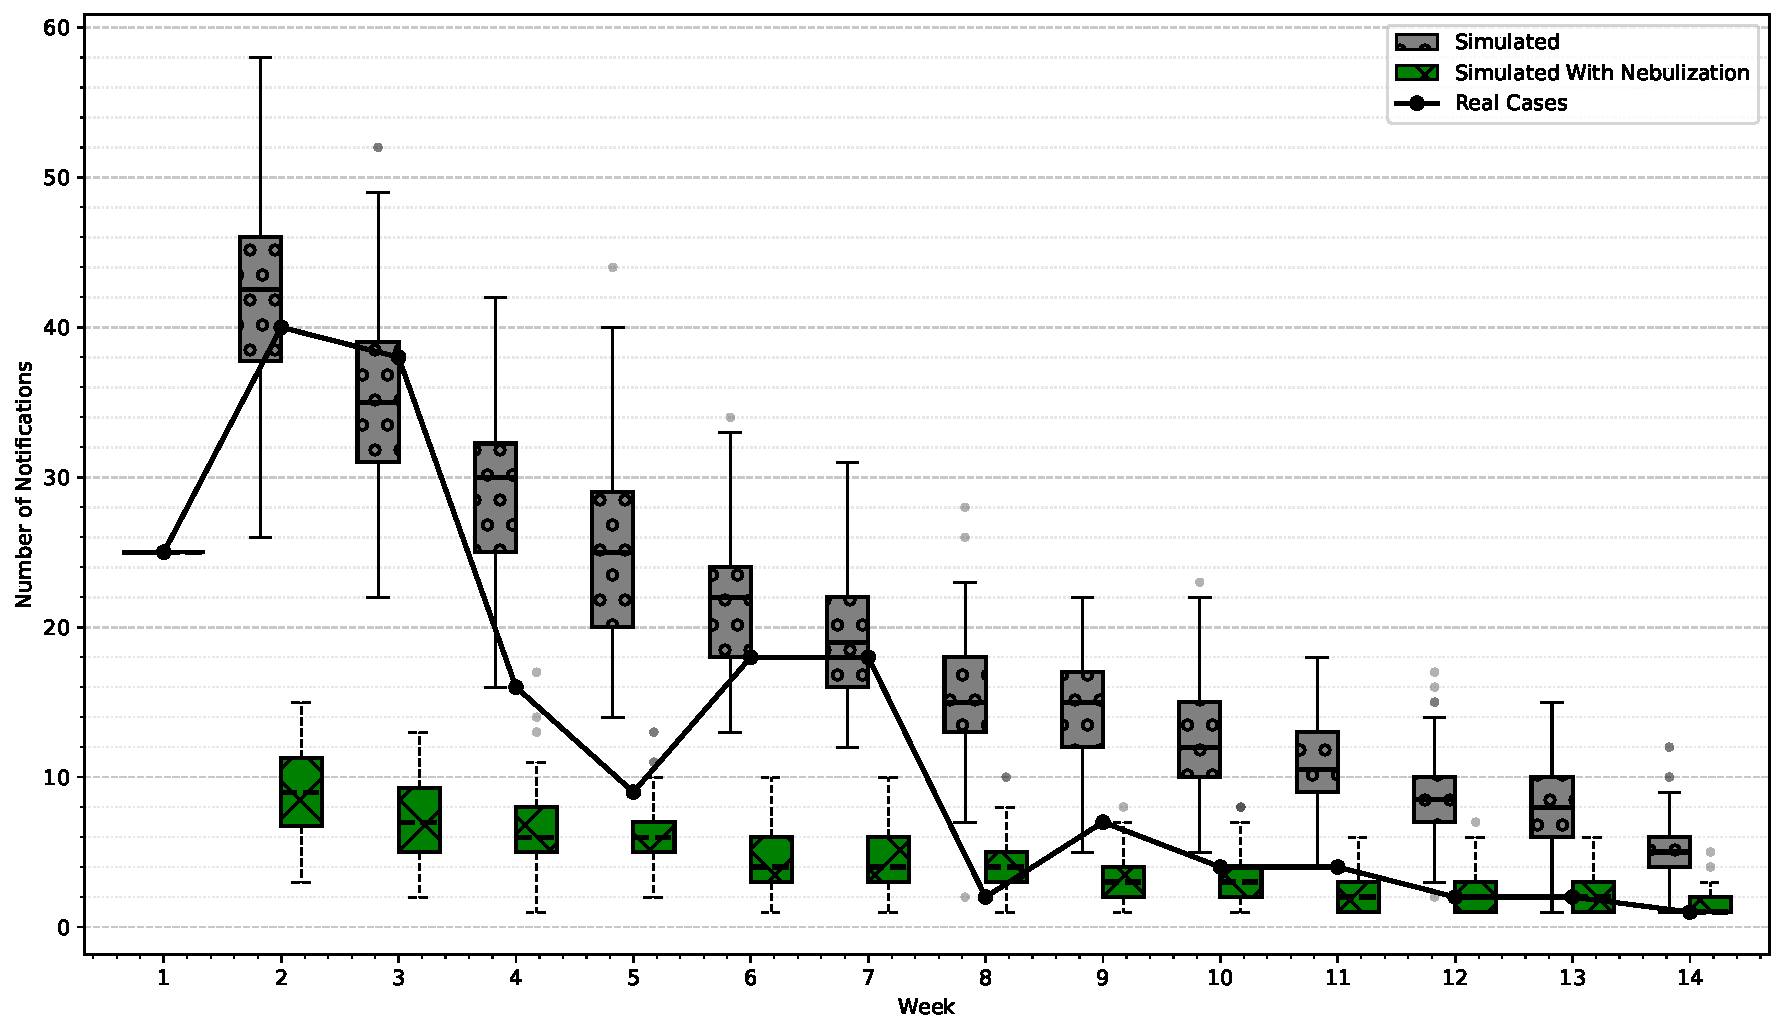
\includegraphics[scale=0.25]{images/action-experiments/as_2017-01-15_weekly_nebulized.pdf} \\
      \subcaption{\label{fig:alto-santo-15-nebulized}Alto Santo - 2017-01-15}
    \end{minipage}
    \hfill
    \begin{minipage}[c]{.45\textwidth}
        \centering
        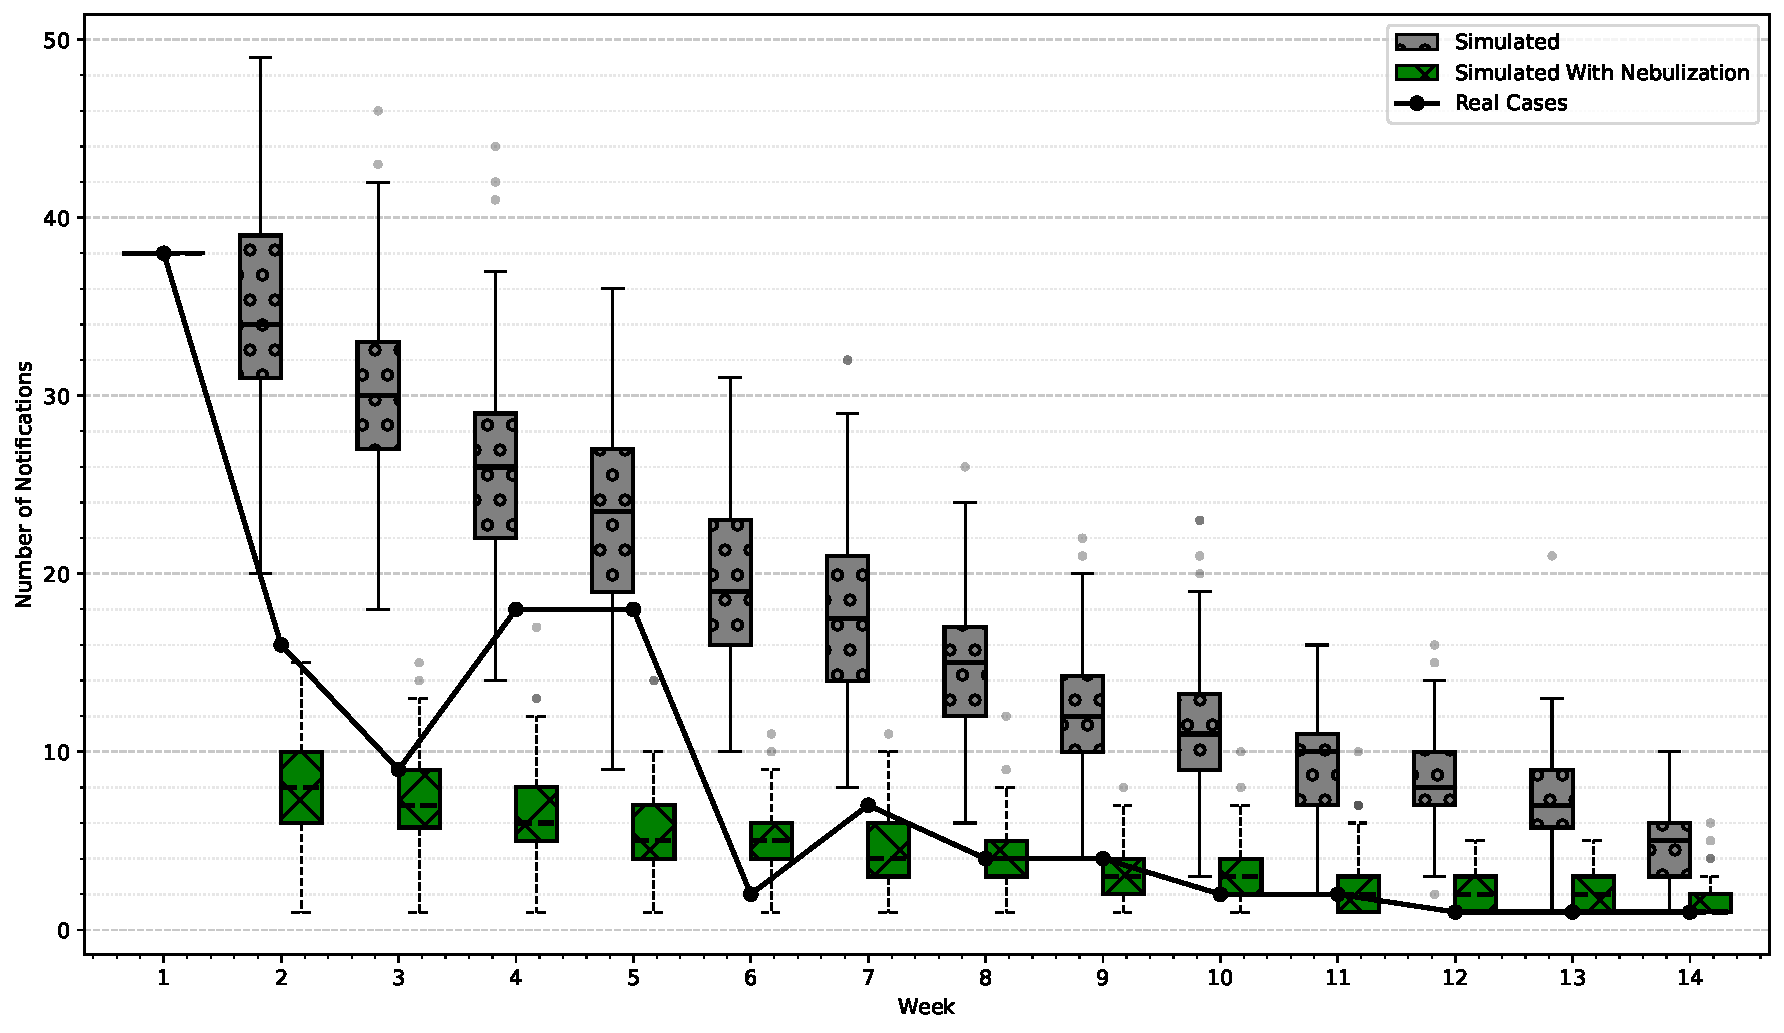
\includegraphics[scale=0.25]{images/action-experiments/as_2017-01-29_weekly_nebulized.pdf} \\
        \subcaption{\label{fig:alto-santo-29-nebulized}Alto Santo - 2017-01-29}
    \end{minipage}
    \caption{\label{fig:emergency-action-impact-as} Estimated Impact of Basic Block Selection Procedure in Alto Santo notifications.}
\end{figure}

\begin{figure}[h!]
    \begin{minipage}[c]{.45\textwidth}
      \centering
      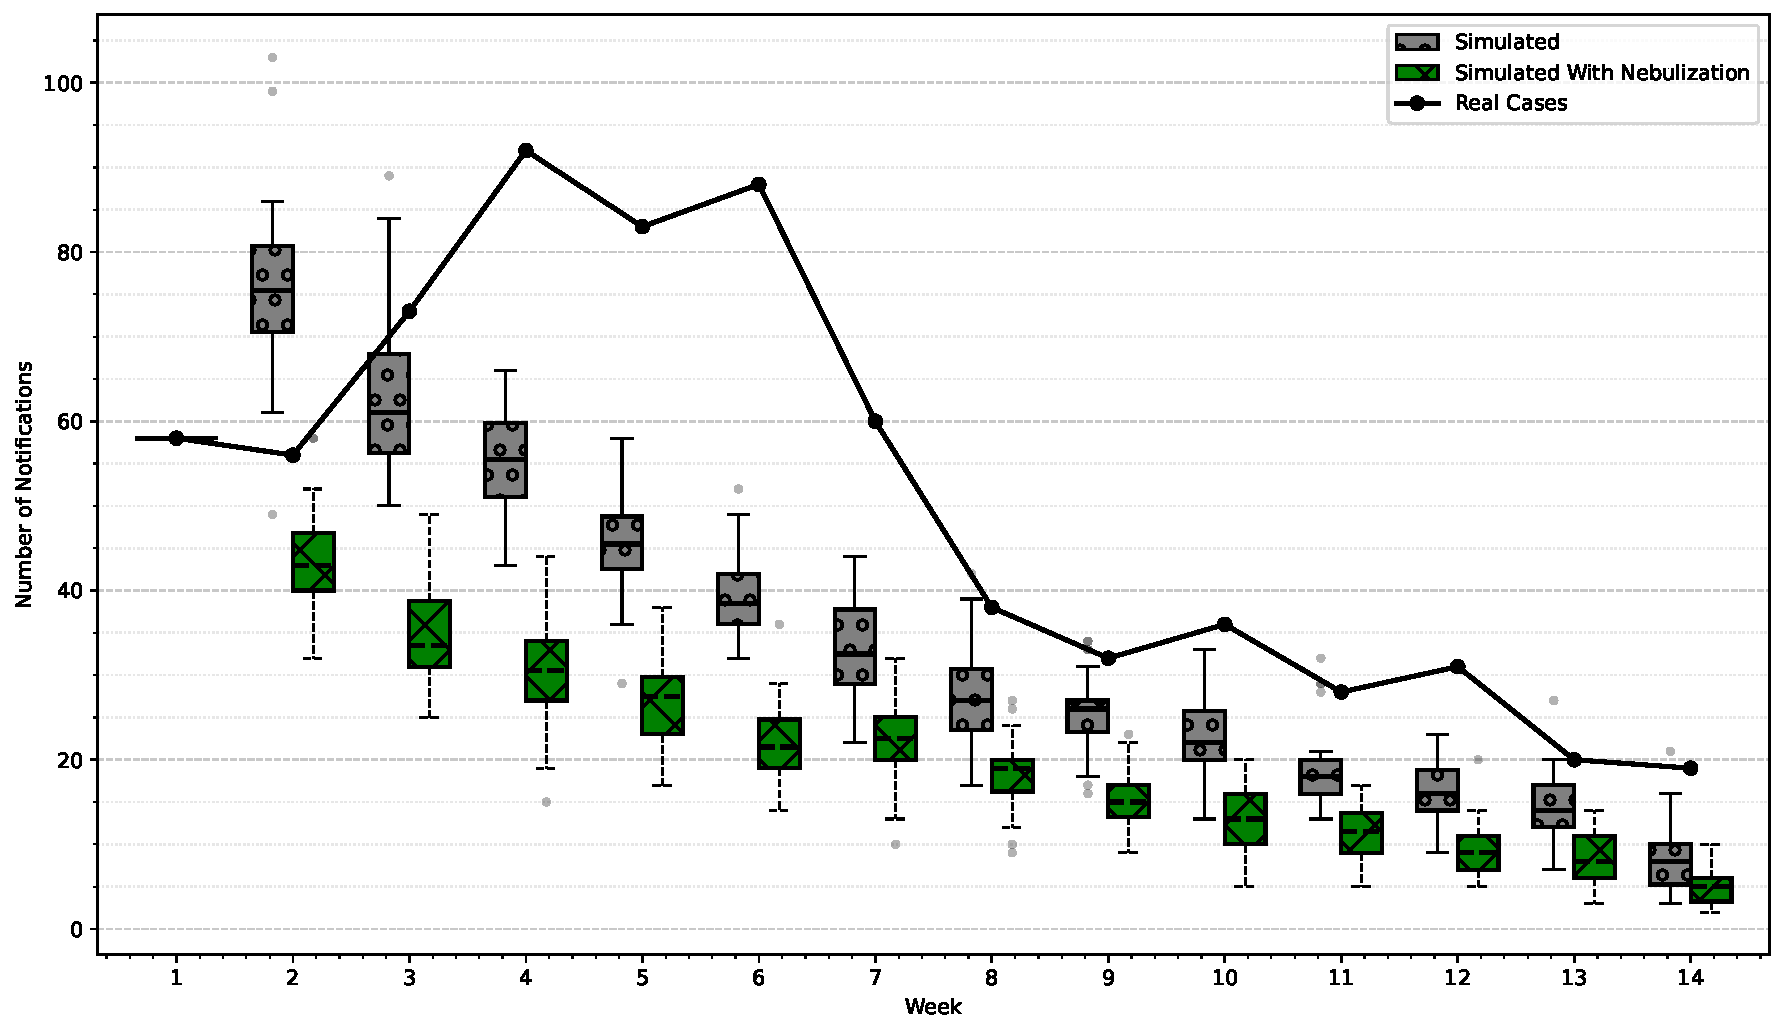
\includegraphics[scale=0.25]{images/action-experiments/lm_2020-07-05_weekly_nebulized.pdf} \\
      \subcaption{\label{fig:limoeiro-05-nebulized}Limoeiro do Norte - 2020-07-05}
    \end{minipage}
    \hfill
    \begin{minipage}[c]{.45\textwidth}
        \centering
        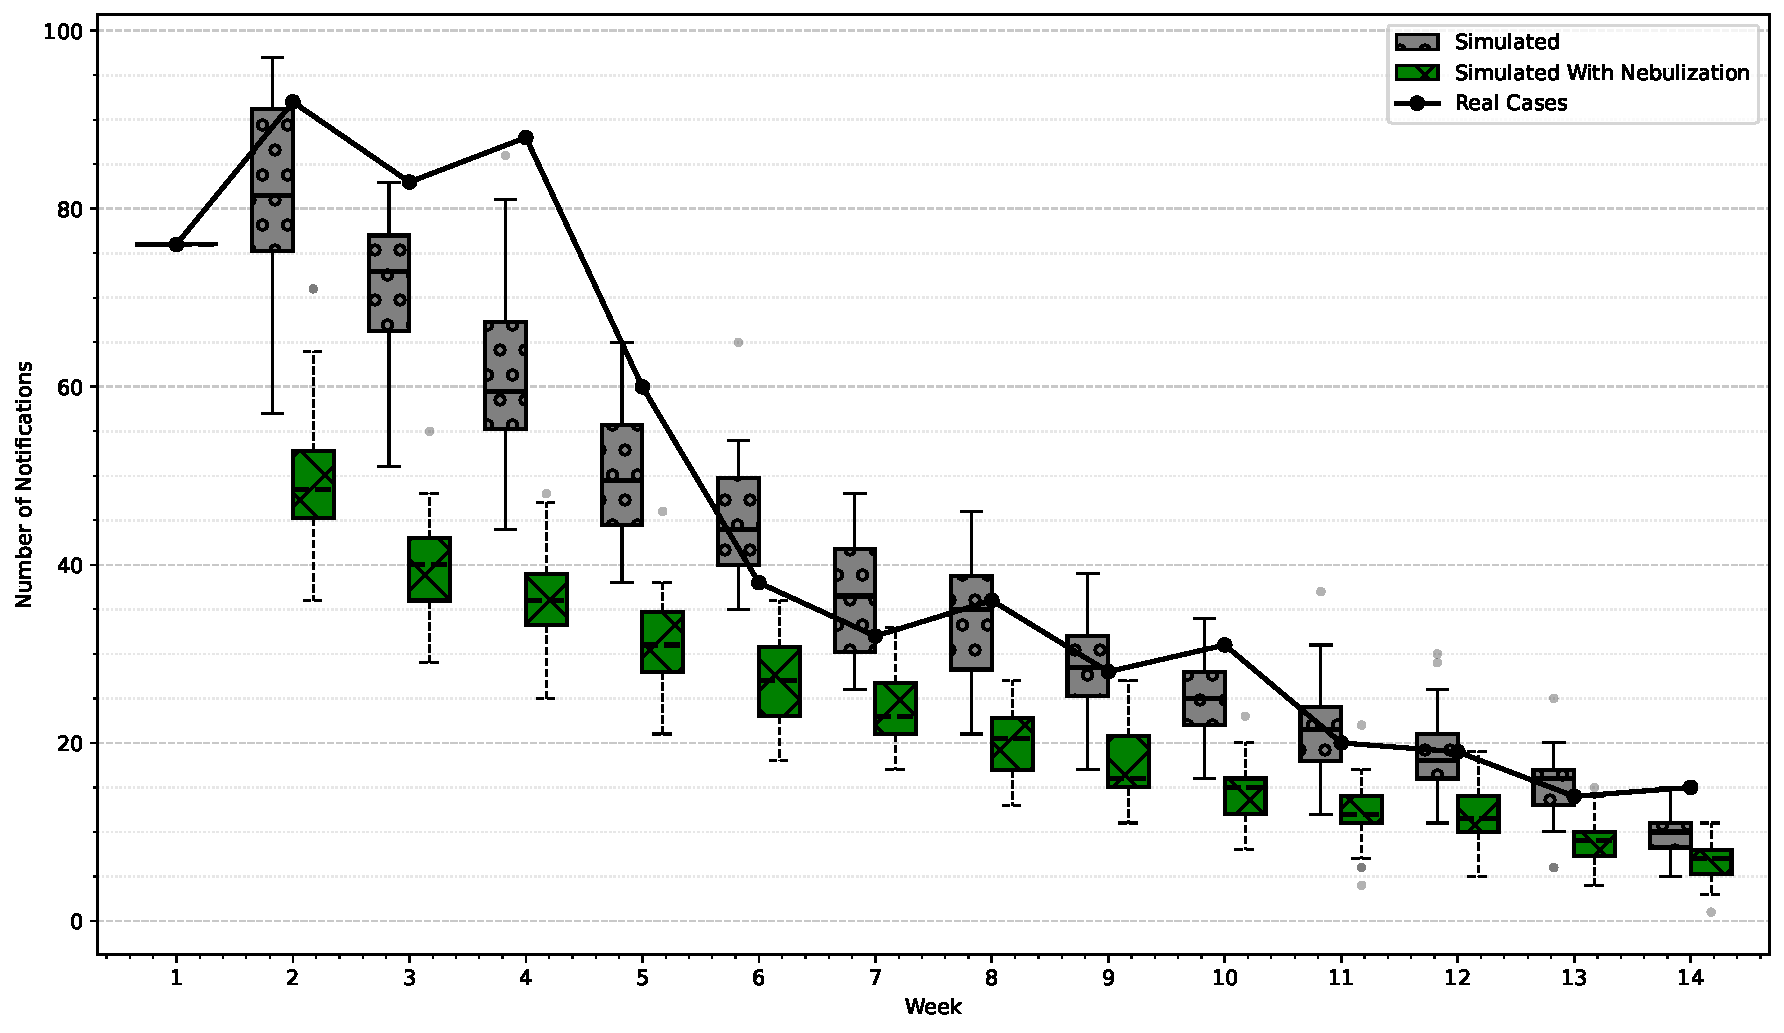
\includegraphics[scale=0.25]{images/action-experiments/lm_2020-07-19_weekly_nebulized.pdf} \\
        \subcaption{\label{fig:limoeiro-19-nebulized}Limoeiro do Norte - 2020-07-15}
    \end{minipage}
    \caption{\label{fig:emergency-action-impact-lm} Estimated Impact of Basic Block Selection Procedure in Limoeiro do Norte notifications.}
\end{figure}

\subsection{Model Performance and Assumptions}

Taking into account all the results presented, it is possible to highlight the strengths of our \gls{mabs} that achieve good results for all simulations in \textit{Alto Santo}. These outcomes present a strong correlation for all cases and a good fit of the real data inside the simulated endemic channel.
The \gls{mabs} also presents a strong correlation for half of the simulations for \textit{Limoeiro} and a good adjustment of the endemic channel to contain the historical progression of notifications. 

In some instances, the simulation's inability to accurately capture real-world data may be attributed to unmodeled factors. For example, the model currently does not account for the influence of climate, vector control efforts, under-reporting, population density, and geographic features like vacant land and proximity to water bodies. These factors can significantly impact disease transmission dynamics, however, may not be fully represented in the current simulation model.

Although the current \gls{mabs} framework cannot dynamically adapt parameters in response to real-time data, it remains a robust analytical tool when combined with the calibration of strategic parameters and domain expertise. By integrating the principles of \gls{mabs} with epidemiological insights specific to dengue transmission, researchers can identify optimal parameter configurations that produce highly accurate simulations. Inclusion of real-time data streams or detailed geographic information could further improve the precision of the model. However, such enhancements are not prerequisites for generating meaningful results.

Thus, it is possible to claim that the proposed \gls{mabs} is a reliable and accurate simulation methodology, capable of generating scenarios that account for both casual disease spread and endemic seasons in the cities of \textit{Alto Santo} and \textit{Limoeiro}, even with limitations in accurate and essential information. The methodology can be further enhanced with additional data, and the simplified programming language facilitates the integration of new features and information into the \gls{mabs}. This approach can be used as a visualization and decision support tool, primarily considering the generated endemic channel and the fact that it is easy to simulate for other cities assuming the existence of basic geographic information and historical data to improve the best fit of the variable parameters.

\section{Final Remarks}\label{sec:final-remarks}

We developed a Multi-Agent-Based Simulation (\gls{mabs}) to model dengue transmission and evaluated it in the Brazilian cities of \textit{Alto Santo} and \textit{Limoeiro do Norte}. The study sought configurations that best matched historical notifications by exploring parameter combinations and assessing performance over multiple runs using average (min–max) weekly cases, Pearson’s correlation ($r$), Mean Absolute Error (\gls{mae}), and the simulated endemic channel.

The proposed \gls{mabs} achieved strong temporal correlations, indicating an ability to capture trends under varied initial conditions. The model proved effective for scenario-based projections that mirror observed epidemiological patterns while quantifying uncertainty. This capability supports public-health decision-making where budgets are constrained: visualizing plausible outbreak trajectories helps prioritize high-risk areas, allocate resources (e.g., insecticides, medical supplies, community interventions), and adapt strategies dynamically. Coupling the simulation with optimization methods can further structure trade-off analysis and scheduling, maximizing the impact of vector-control actions~\cite{araujo:2022,andrade:2021}.

Looking ahead, extensions can increase realism and decision value while preserving parsimony. A natural step is to couple entomological processes to environmental drivers: temperature, humidity, and rainfall affect survival, reproduction, and viral development~\cite{maneerat:2016,Abidemi2020,hamdan:2021}. Allowing these variables to follow observed or forecast climate would induce seasonality and enable stress tests under extremes; linking breeding-site productivity to rainfall and local conditions (e.g., rivers, shaded areas, small containers) would ground mosquito dynamics ecologically. Additional refinements include explicit gonotrophic cycles and diurnal activity patterns on the vector side, and human heterogeneity in routines, age, or social mixing—along with multiple serotypes and temporary cross-immunity—to capture multi-annual dynamics and secondary-infection risks. Public-health actions (source reduction, larviciding, adulticiding, campaigns) can then be represented explicitly for policy evaluation~\cite{Abidemi2020}.

These gains come with costs: high-quality data are uneven, parameter mapping is delicate, and added mechanisms enlarge the parameter space, complicating calibration and risking overfitting. More realism also increases runtime and can hinder communication. Future work should therefore prioritize extensions by expected benefit per added complexity, keeping a balance between realism and usability so that the tool remains both scientifically rigorous and operationally useful for early warning and proactive arboviral disease management.
